% !TEX root = perelman-geometry.tex
%!TEX TS-program = pdflatex
%!TEX encoding = UTF-8 Unicode

\setchapterpreamble[o]{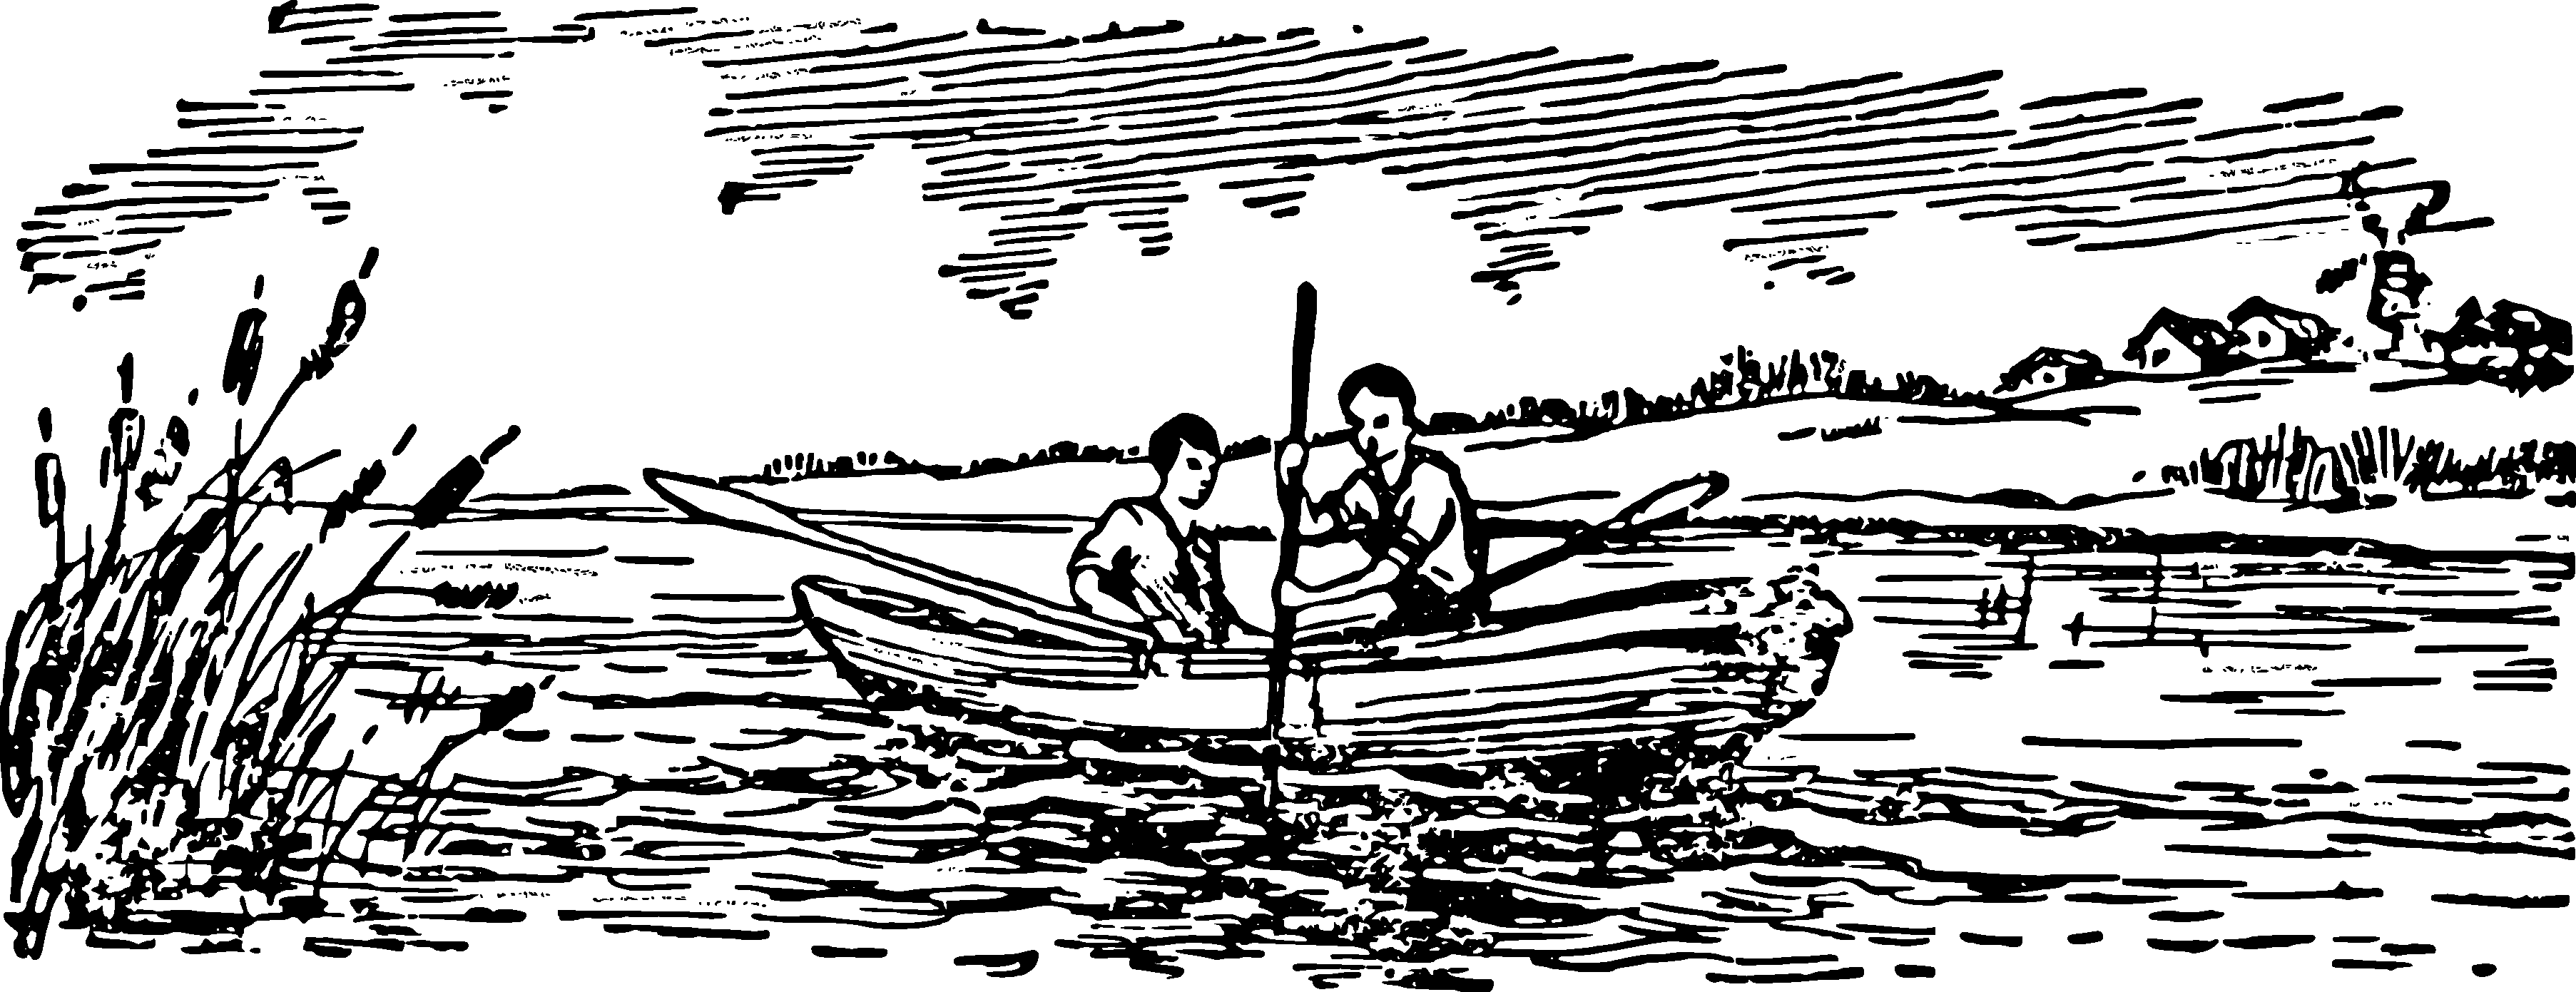
\includegraphics[width=1.2\textwidth]{figures/ch-02/fig-ch-02-head.pdf}\bigskip}

\chapter{Geometry By The River}
\label{ch-02}

\section{Measuring the width of the river}
\label{sec-2.1}
When crossing a river, measuring its width is just as easy for those who know geometry, how to determine the height of a tree, without climbing to the top. The inaccessible distance is measured the same techniques that we used to measure the inaccessible height. In both cases, the definition of the desired distance is replaced an example of another distance that is easily measurable directly.

Of the many ways to solve this problem, let's look at some of the simplest ones.

\begin{figure}[h!]
\centering
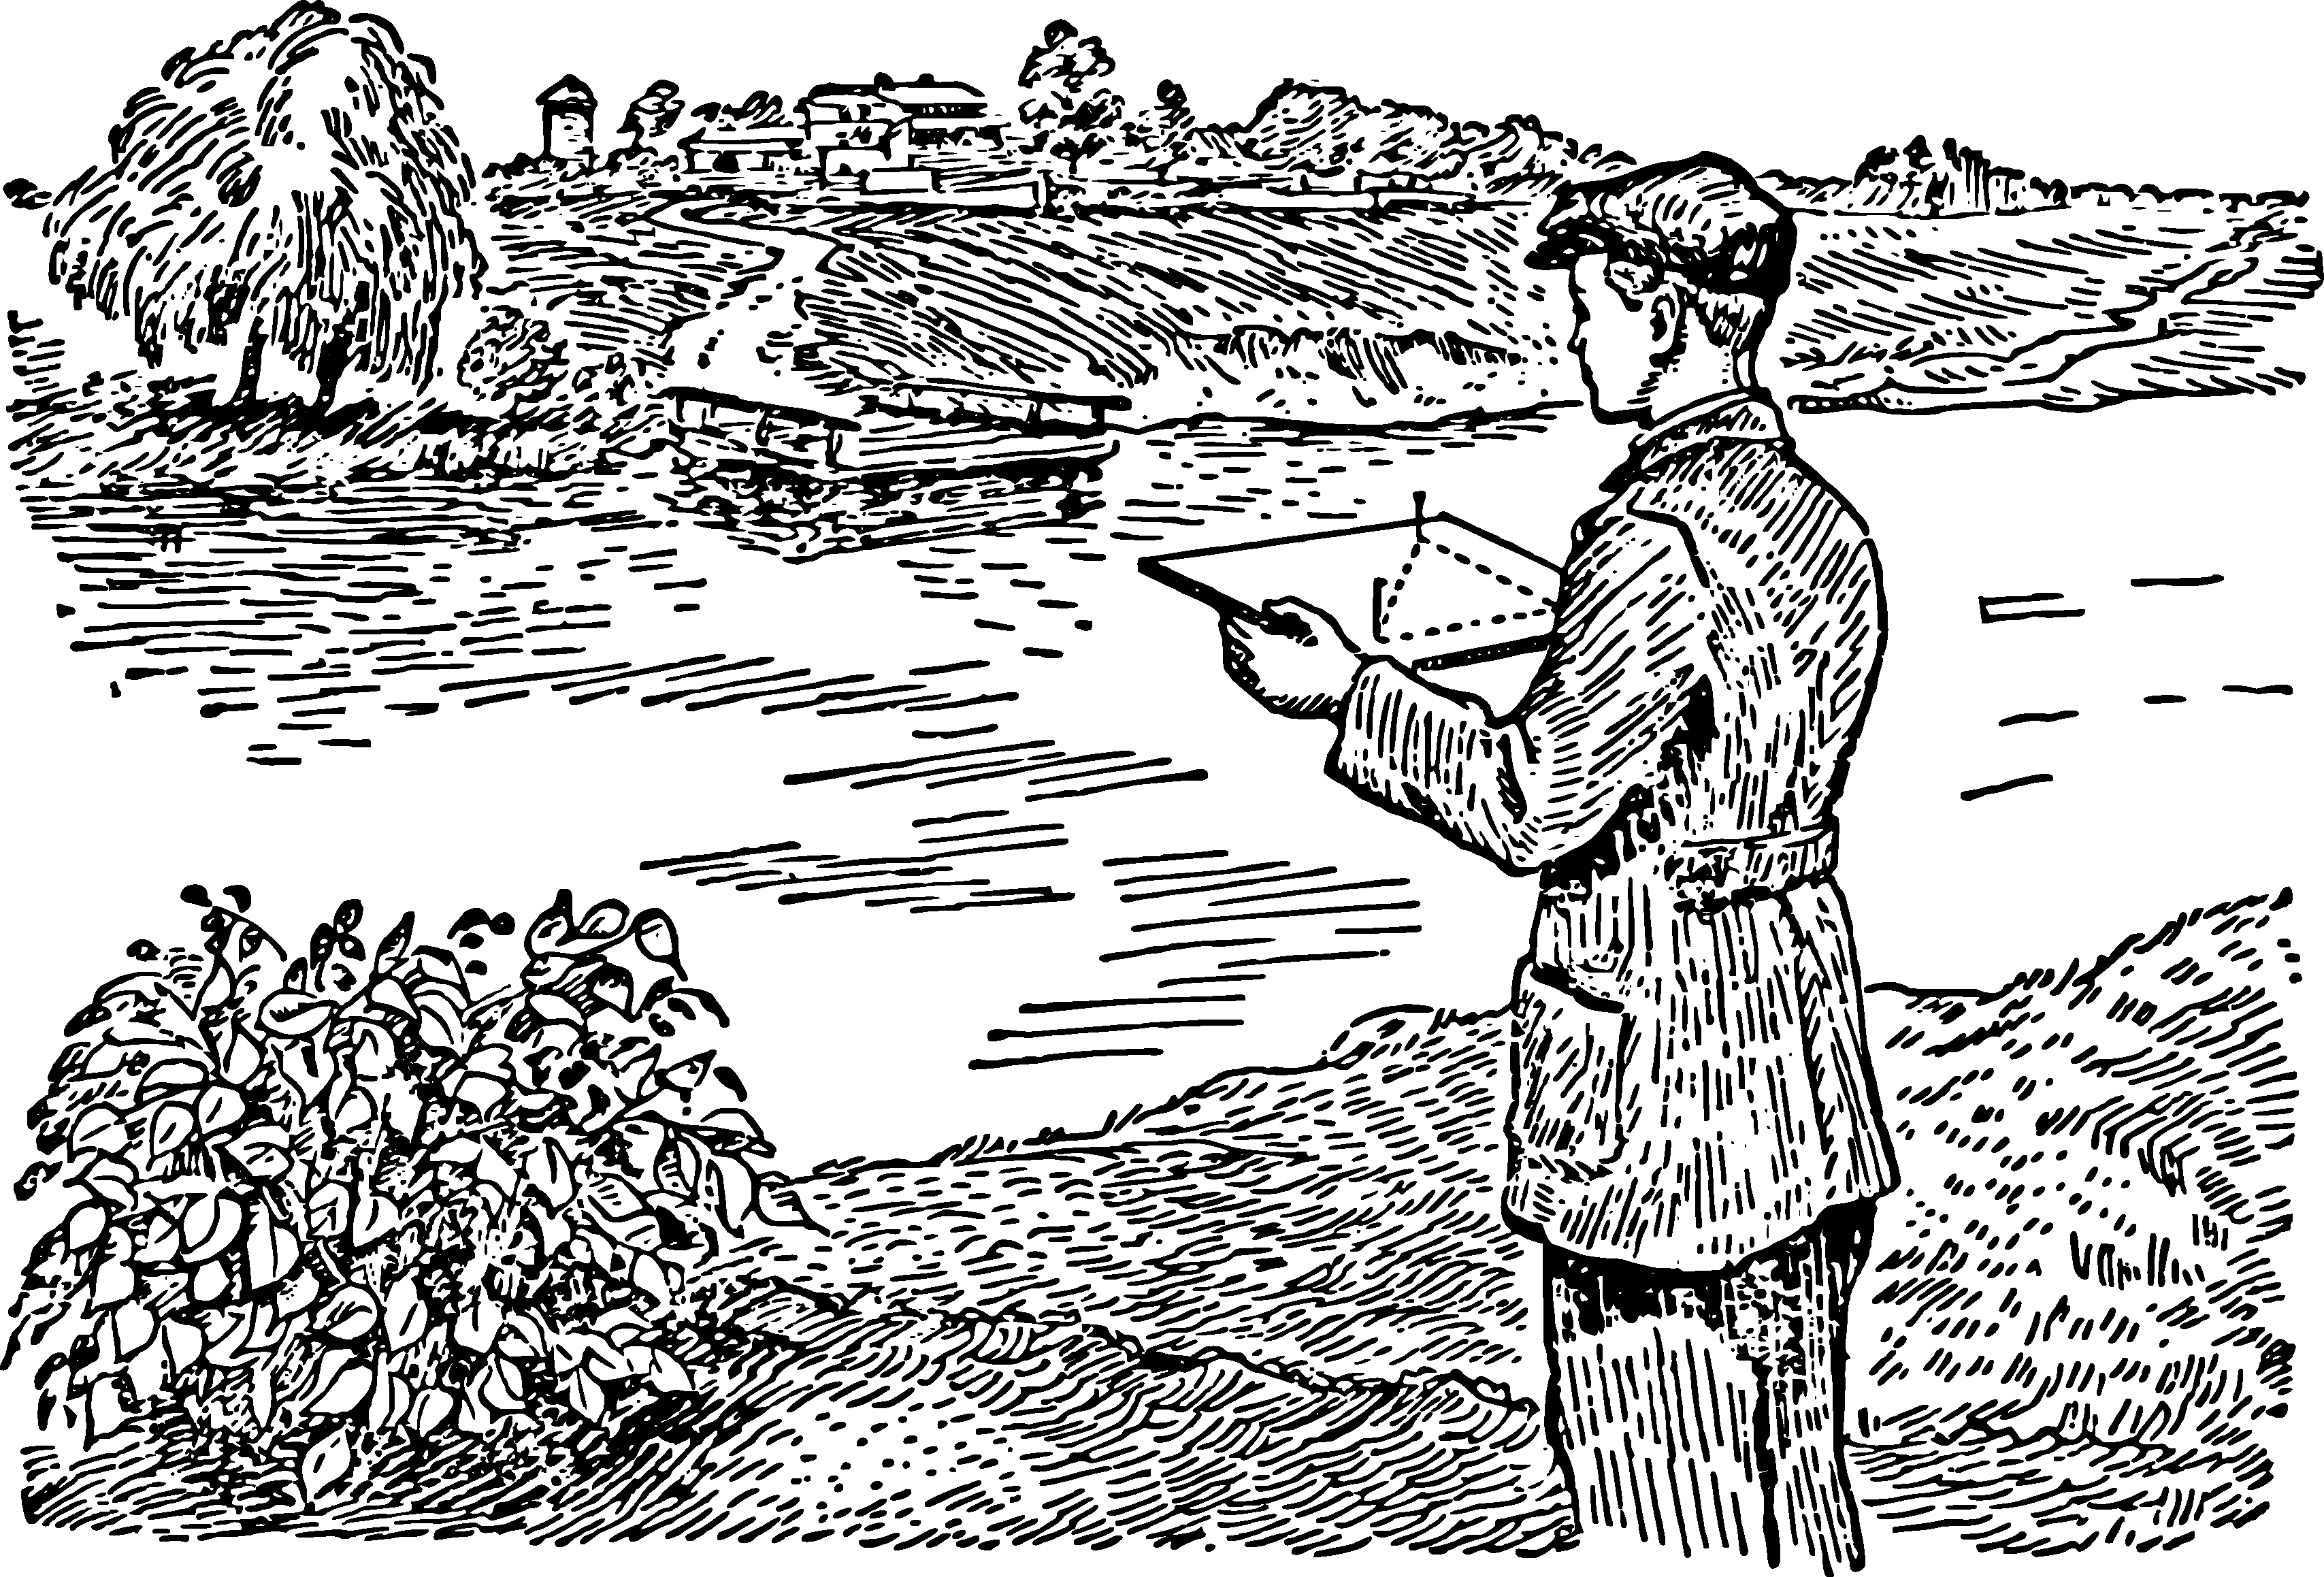
\includegraphics[width=0.9\textwidth]{figures/ch-02/fig-025.pdf}
\sidecaption{Measuring the width of the river with a pin device.\label{fig-025}}
\end{figure}

\begin{enumerate}
\item The first method requires the familiar ``device'' with three pins at the vertices of an isosceles right triangle (\figr{fig-025}). 
Let's say we need to determine the width of river $AB$ (\figr{fig-026}), standing on the bank where point $B$ is, without crossing to the opposite bank. Standing somewhere at point $C$, hold the pin device close to your eye so that, looking with one eye along the two pins, you see both covering points $B$ and $A$. It's clear that when you manage this, you will be exactly on the extension of line $AB$. 

\begin{marginfigure}[-1.5cm]%[h!]
\centering
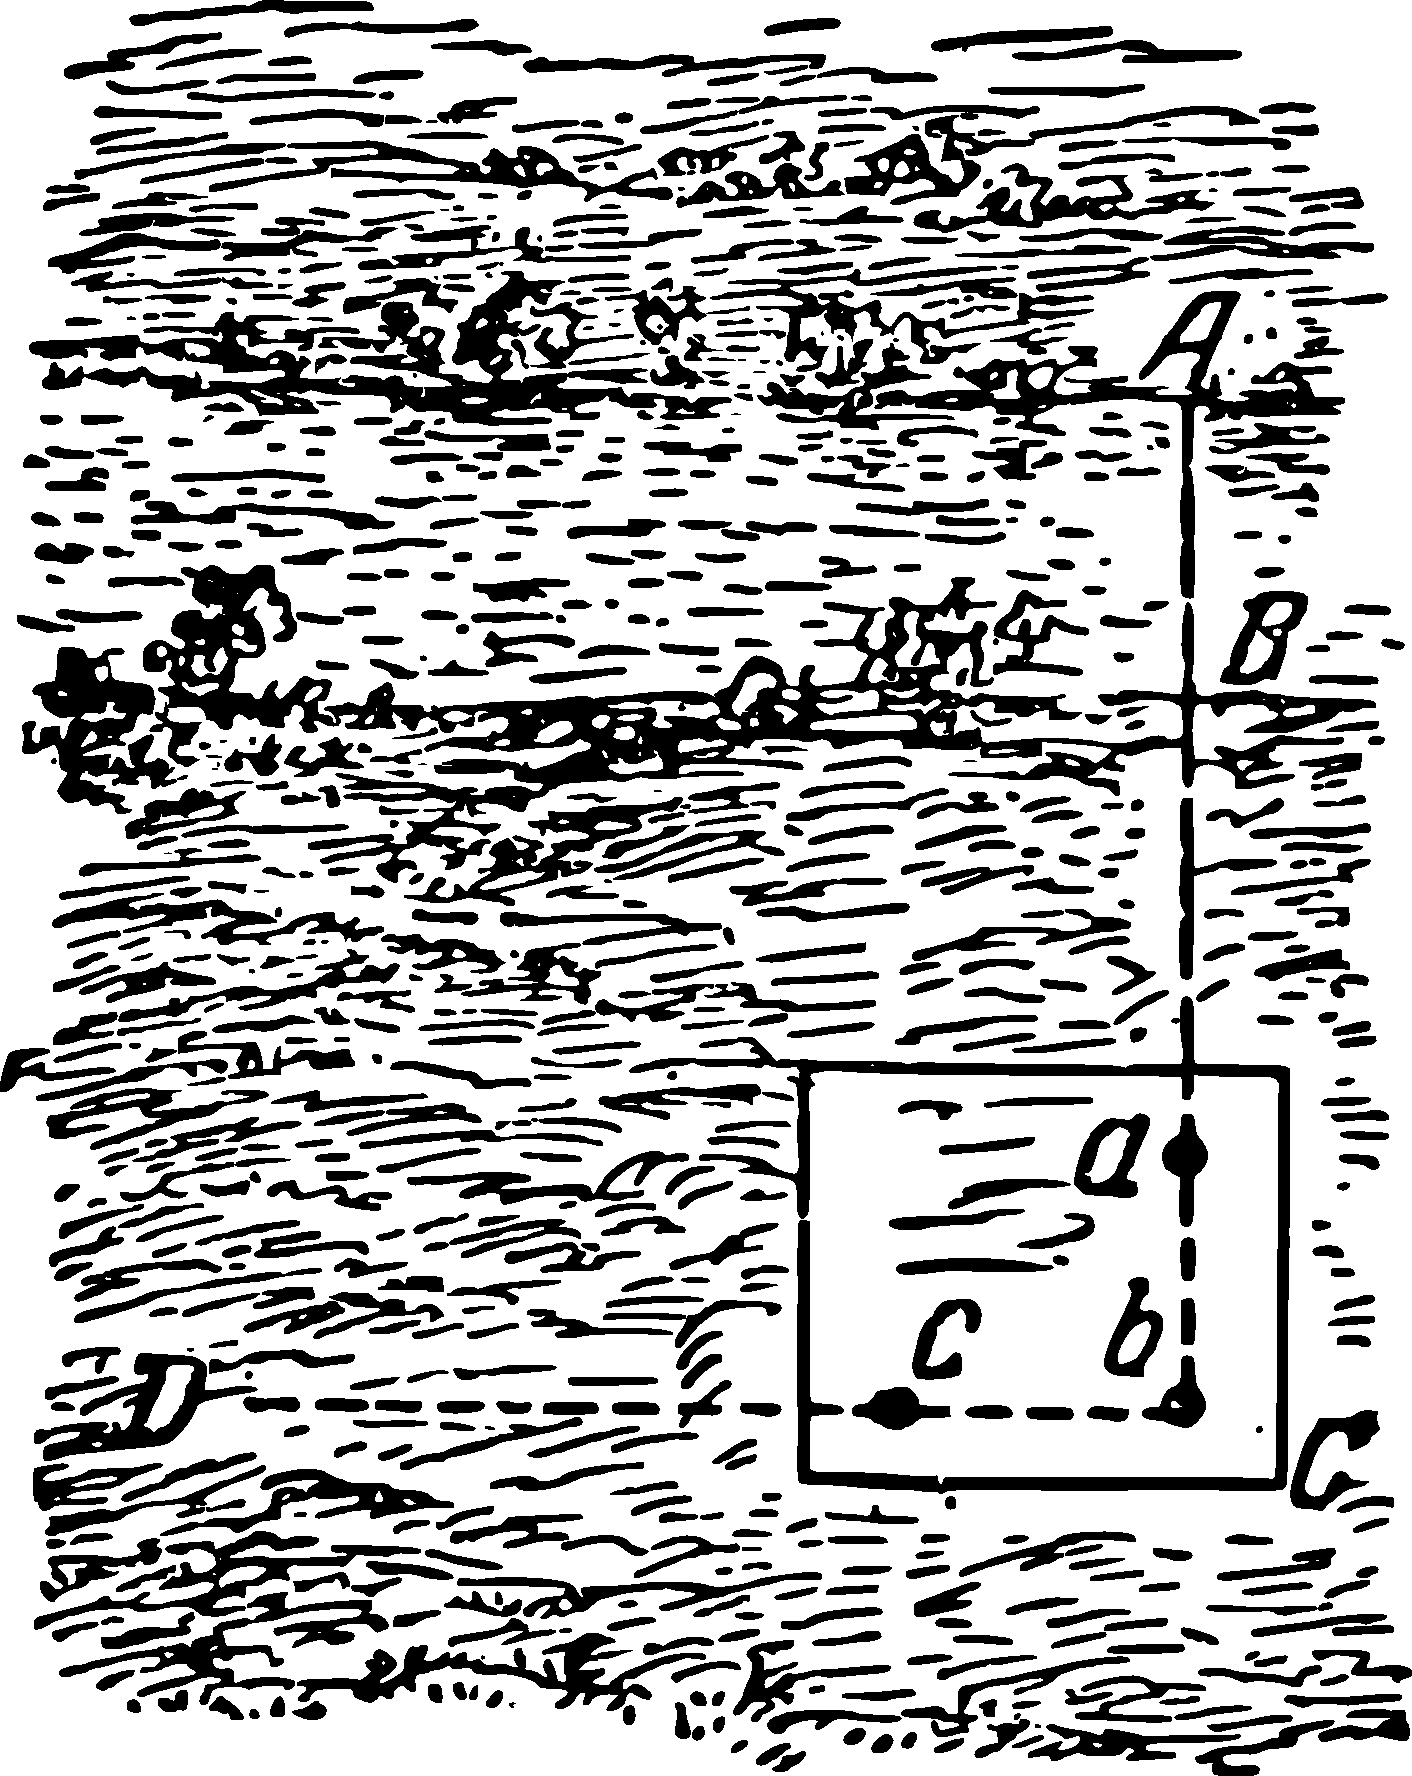
\includegraphics[width=\textwidth]{figures/ch-02/fig-026.pdf}
\sidecaption{First position of the pin device.\label{fig-026}}
\end{marginfigure}
\begin{marginfigure}[5cm]%[h!]
\centering
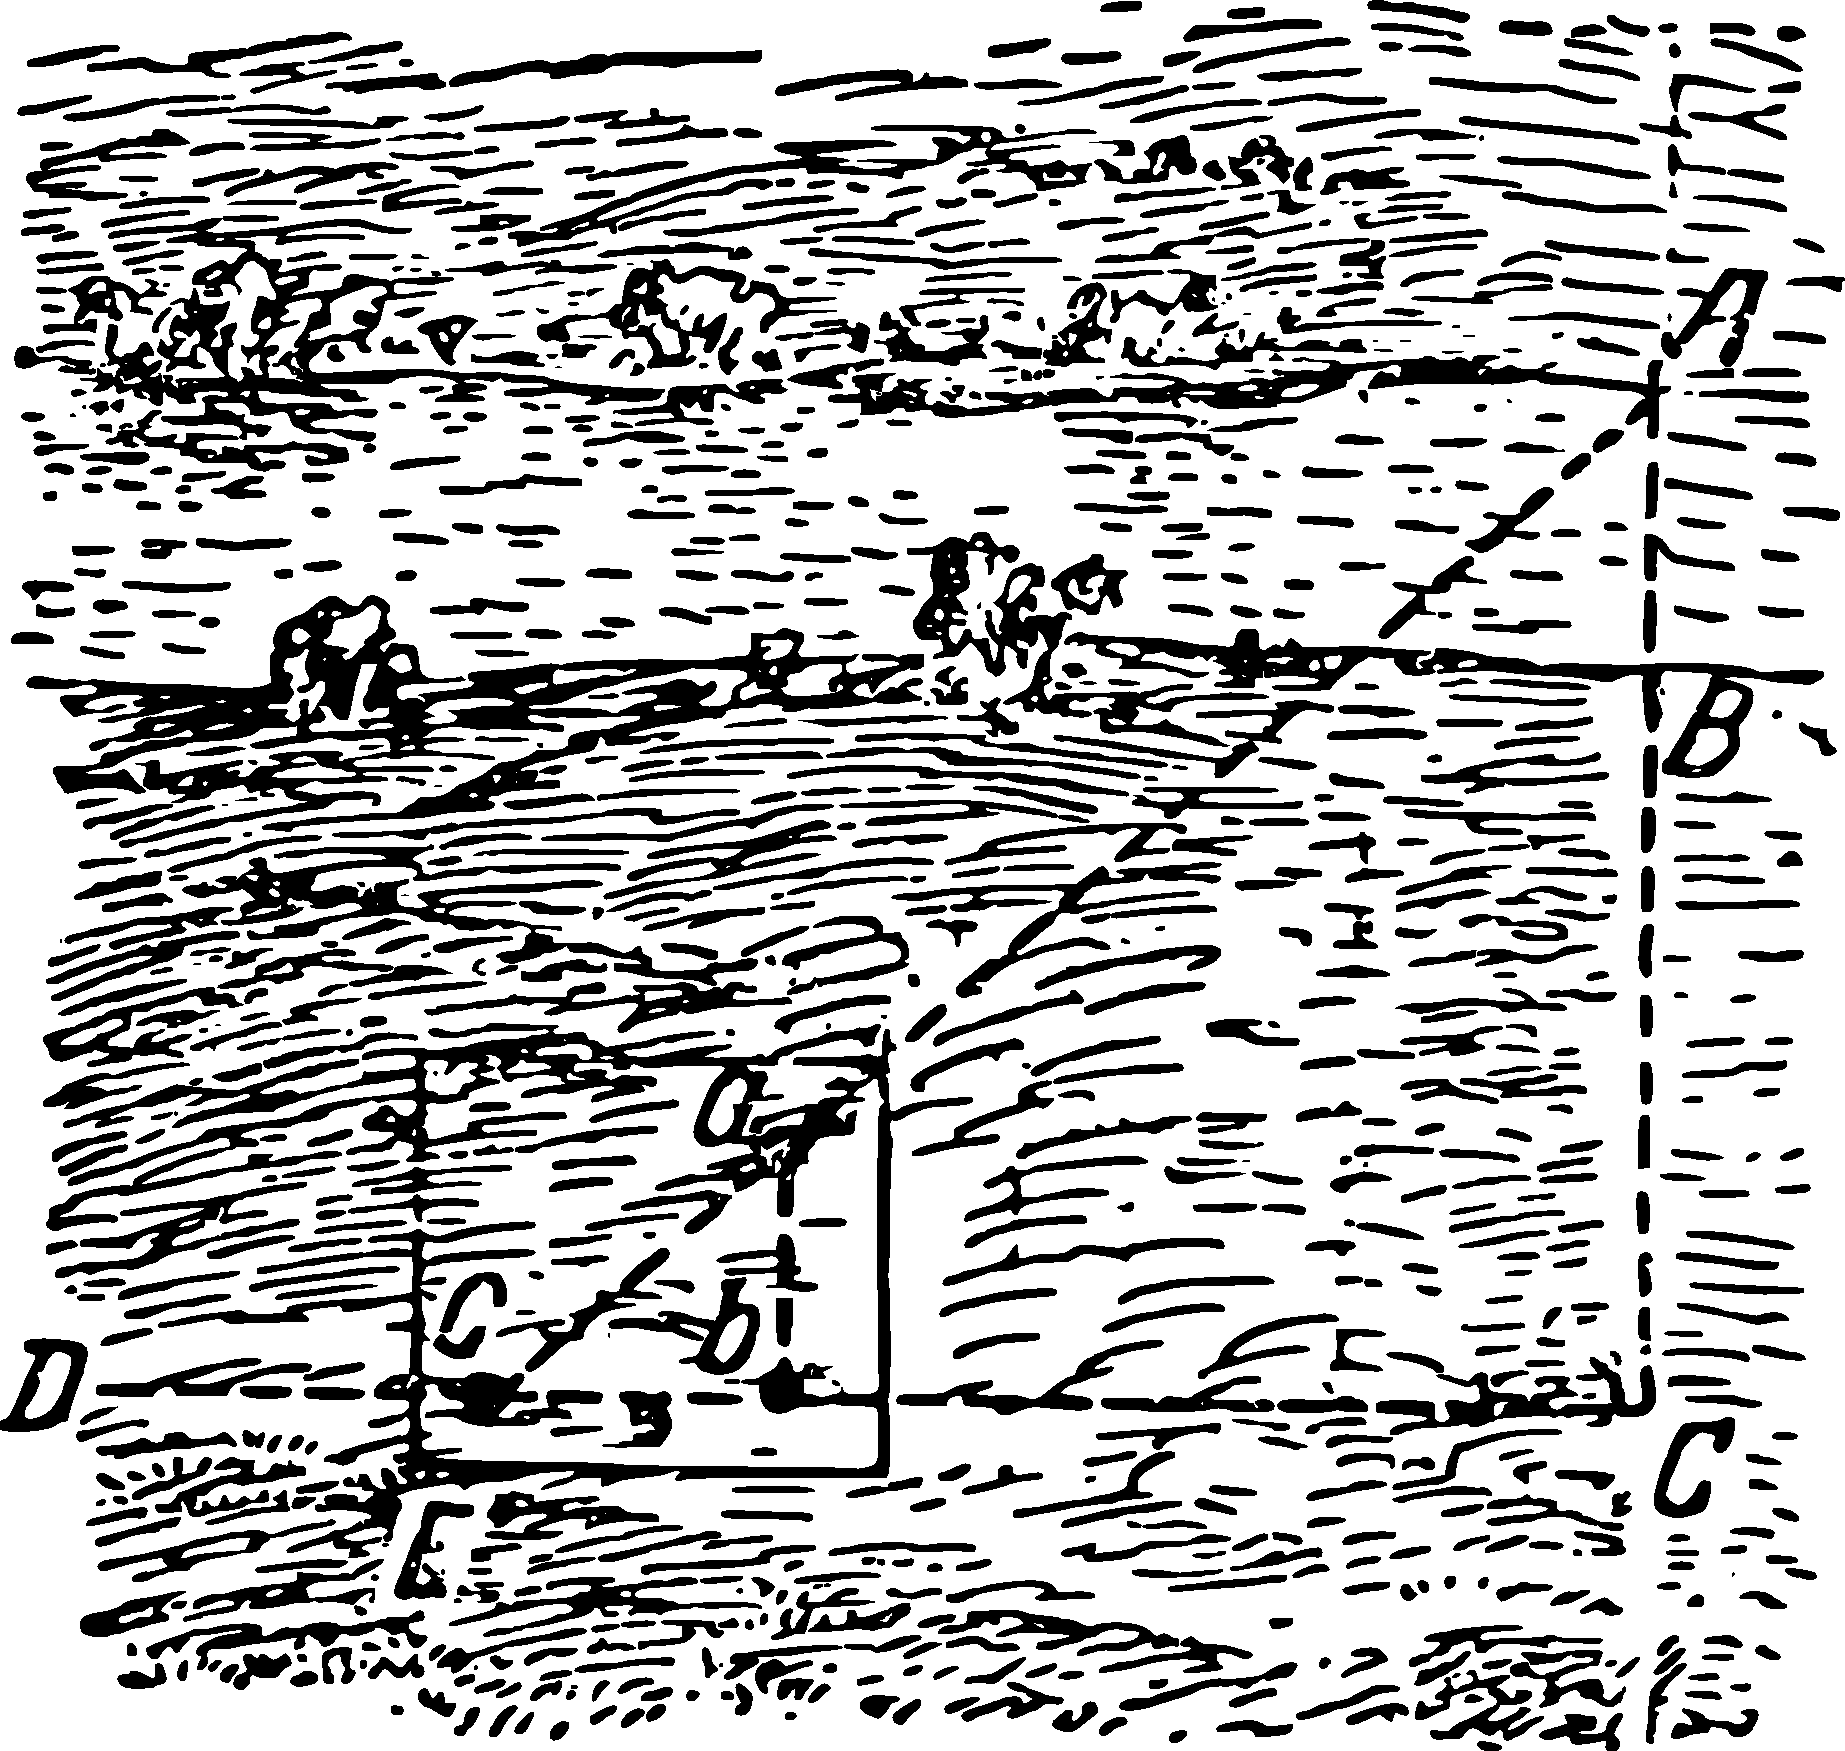
\includegraphics[width=\textwidth]{figures/ch-02/fig-027.pdf}
\sidecaption{Second position of the pin device.\label{fig-027}}
\end{marginfigure}


Now, without moving the plank of the device, look along the other two pins (perpendicular to the previous direction) and notice any point $D$ covered by these pins, i.e., lying on the line perpendicular to $AC$. After this, insert a pin at point $C$, leave this place, and go with your instrument along line $CD$ until you find a point $E$ (\figr{fig-027}), where you can simultaneously cover point $C$ for one eye with pin $b$ and point $A$ with pin $a$. This means you have found the third vertex of triangle $ACE$ on the shore, where angle $C$ is a right angle, and angle $E$ is opposite to the acute angle of the pin device, i.e., half the right angle (\ang{45}). Obviously, angle $A$ is also half right angle, i.e., $AC = CE$. If you measure the distance $CE$ even by steps, you will know the distance $AC$, and by subtracting $BC$, which is easy to measure, you will determine the desired width of the river.

It is quite inconvenient and difficult to hold the pin device still in hand; therefore, it is better to attach this plank to a stick with a pointed end and insert it vertically into the ground.

\item The second method is similar to the first. Here also, find point $C$ on the extension of $AB$ and mark line $CD$ perpendicular to $CA$ using the pin device. But then proceed differently (\figr{fig-028}). Equal distances $CE$ and $EF$ of arbitrary length are measured on the straight line $CD$, and pegs are inserted at points $E$ and $F$. Then, standing at point $F$ with a pin device, the direction $FG$ is marked out perpendicular to $FC$. Now, walking along $FG$, find a point $H$ on this line from which point $A$ seems to be covered by point $E$. This will mean that points $H$, $E$, and $A$ lie on the same straight line.

\begin{figure}[h!]
\centering
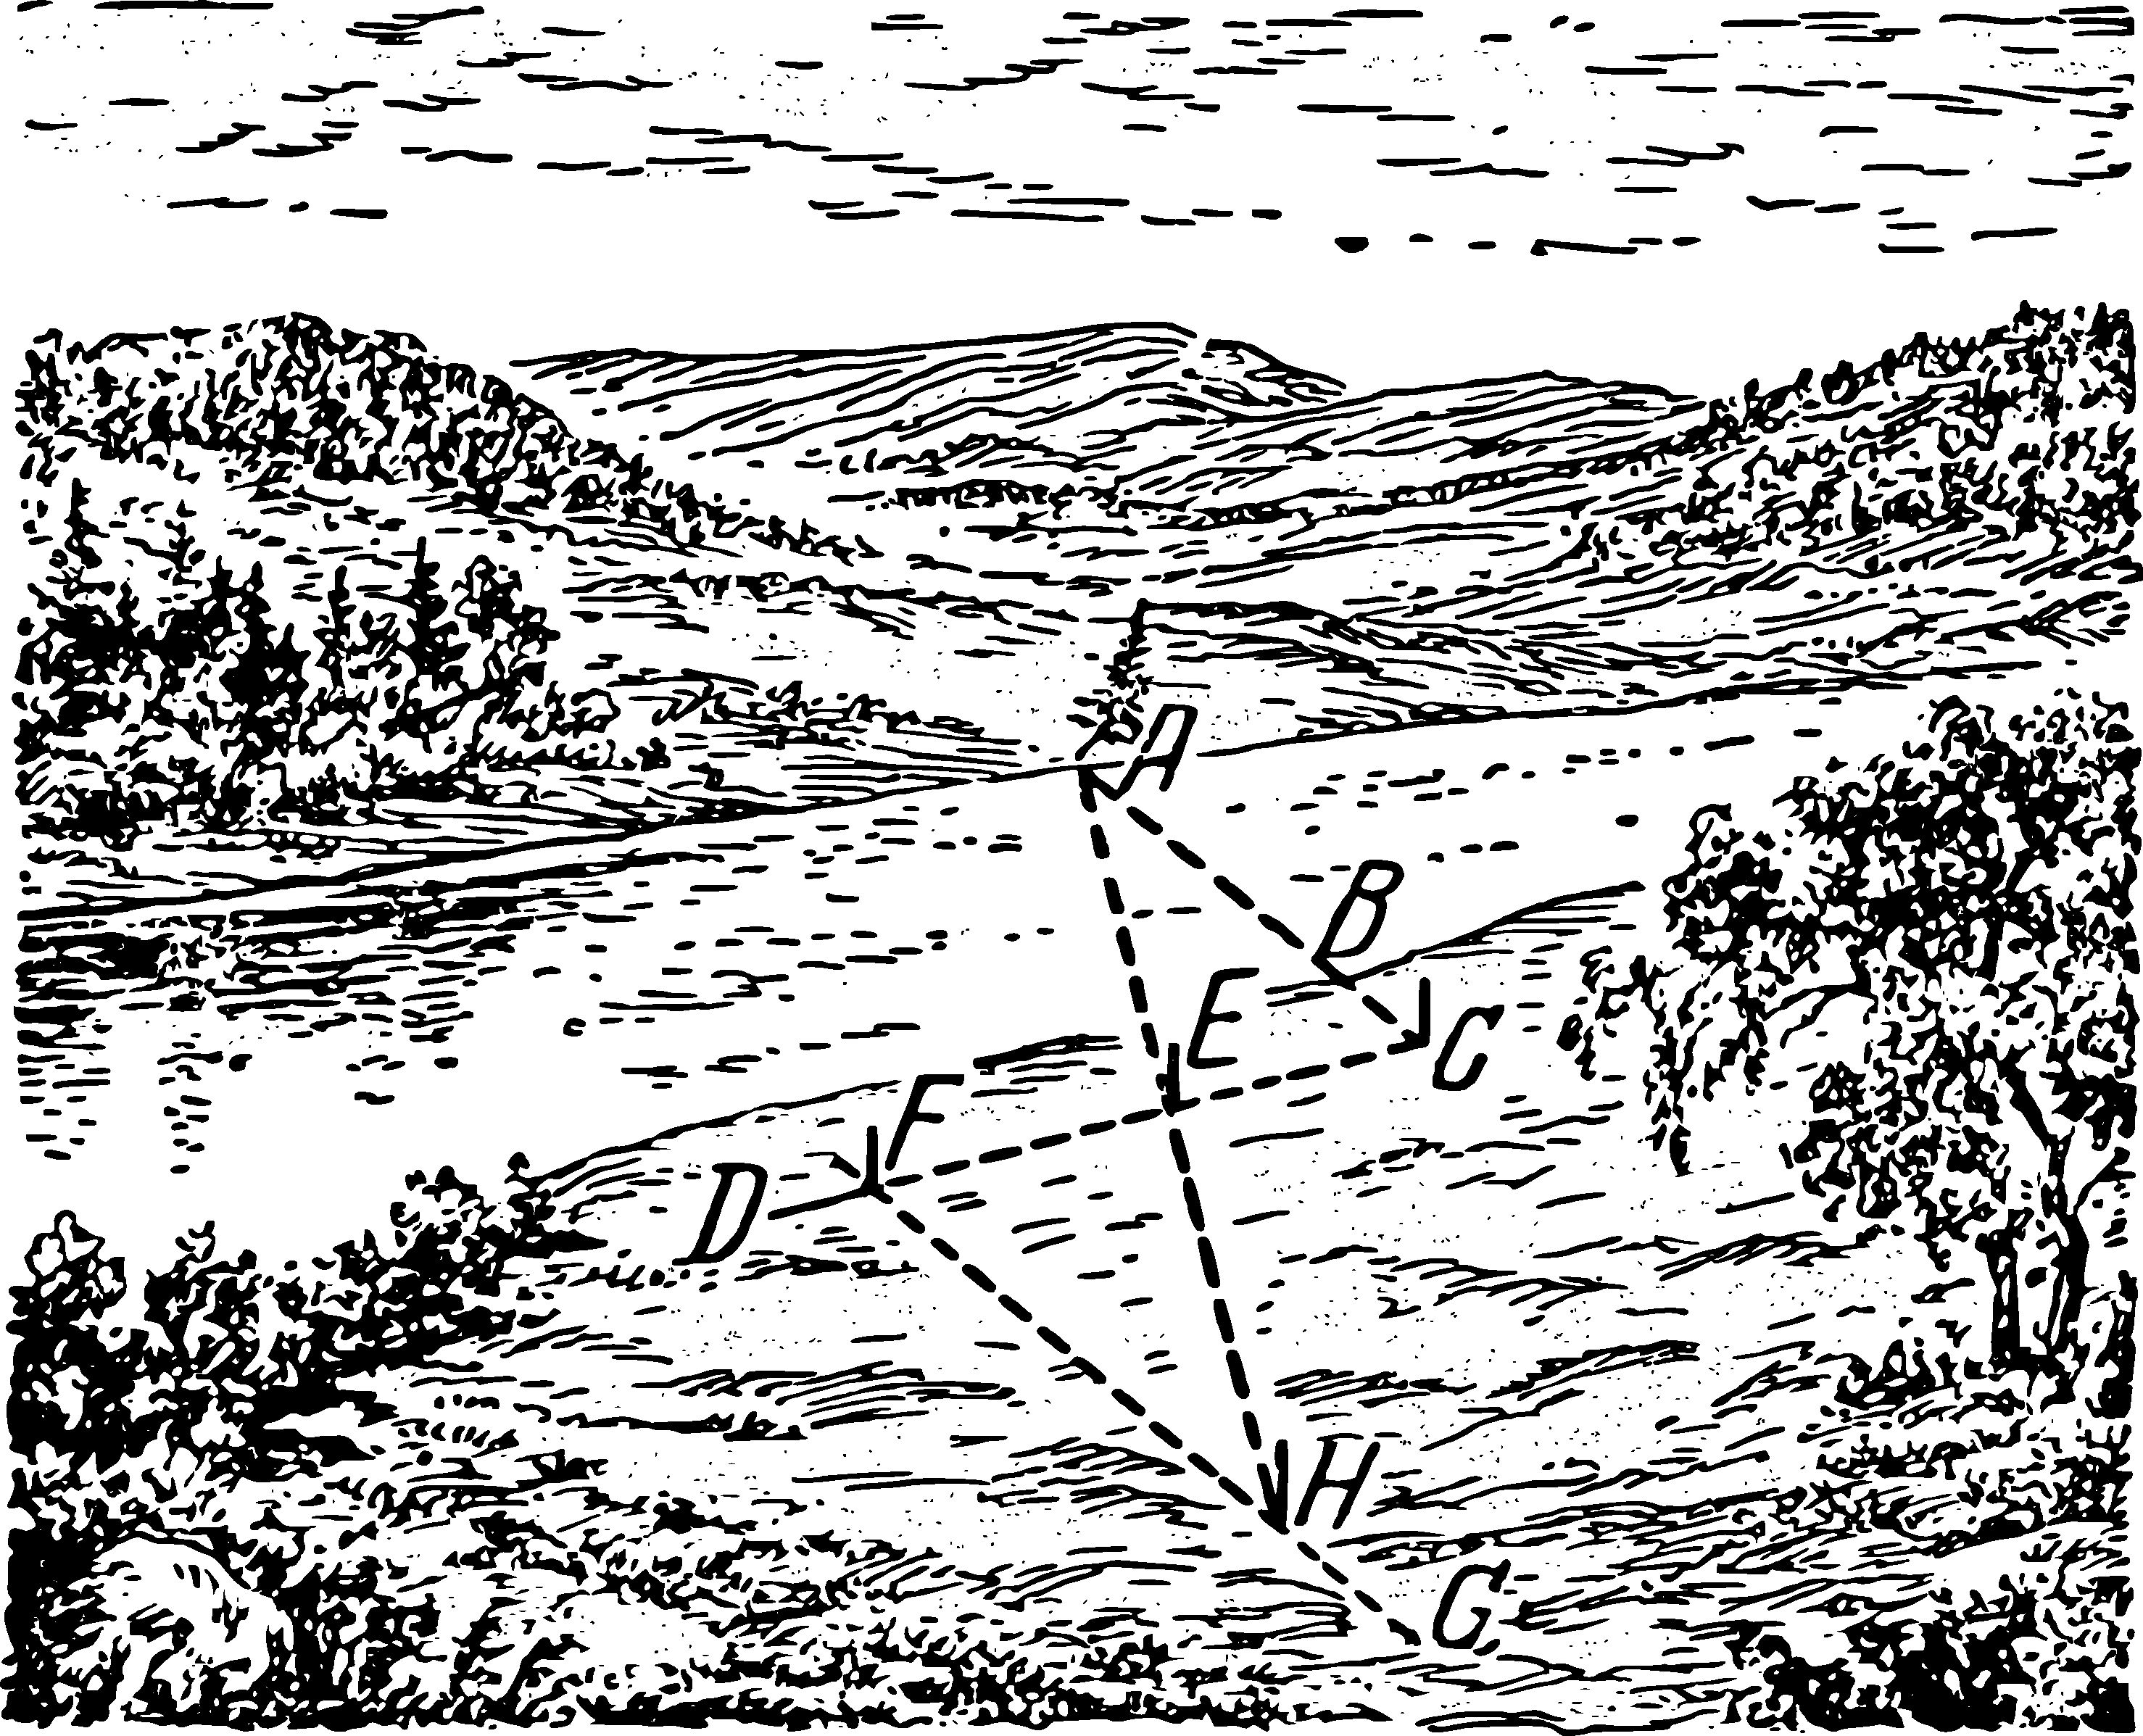
\includegraphics[width=0.9\textwidth]{figures/ch-02/fig-028.pdf}
\sidecaption{ Using the congruence criteria of triangles to find the width of the river.\label{fig-028}}
\end{figure}

The problem is solved: the distance $FH$ is equal to the distance $AC$, from which it is only necessary to subtract $BC$ to find the desired width of the river (the reader, of course, will guess for himself why $FH$ is equal to $AC$).

This method requires more space than the first one; if the terrain allows executing both methods, it is useful to verify one result by another.
\begin{figure}[h!]
\centering
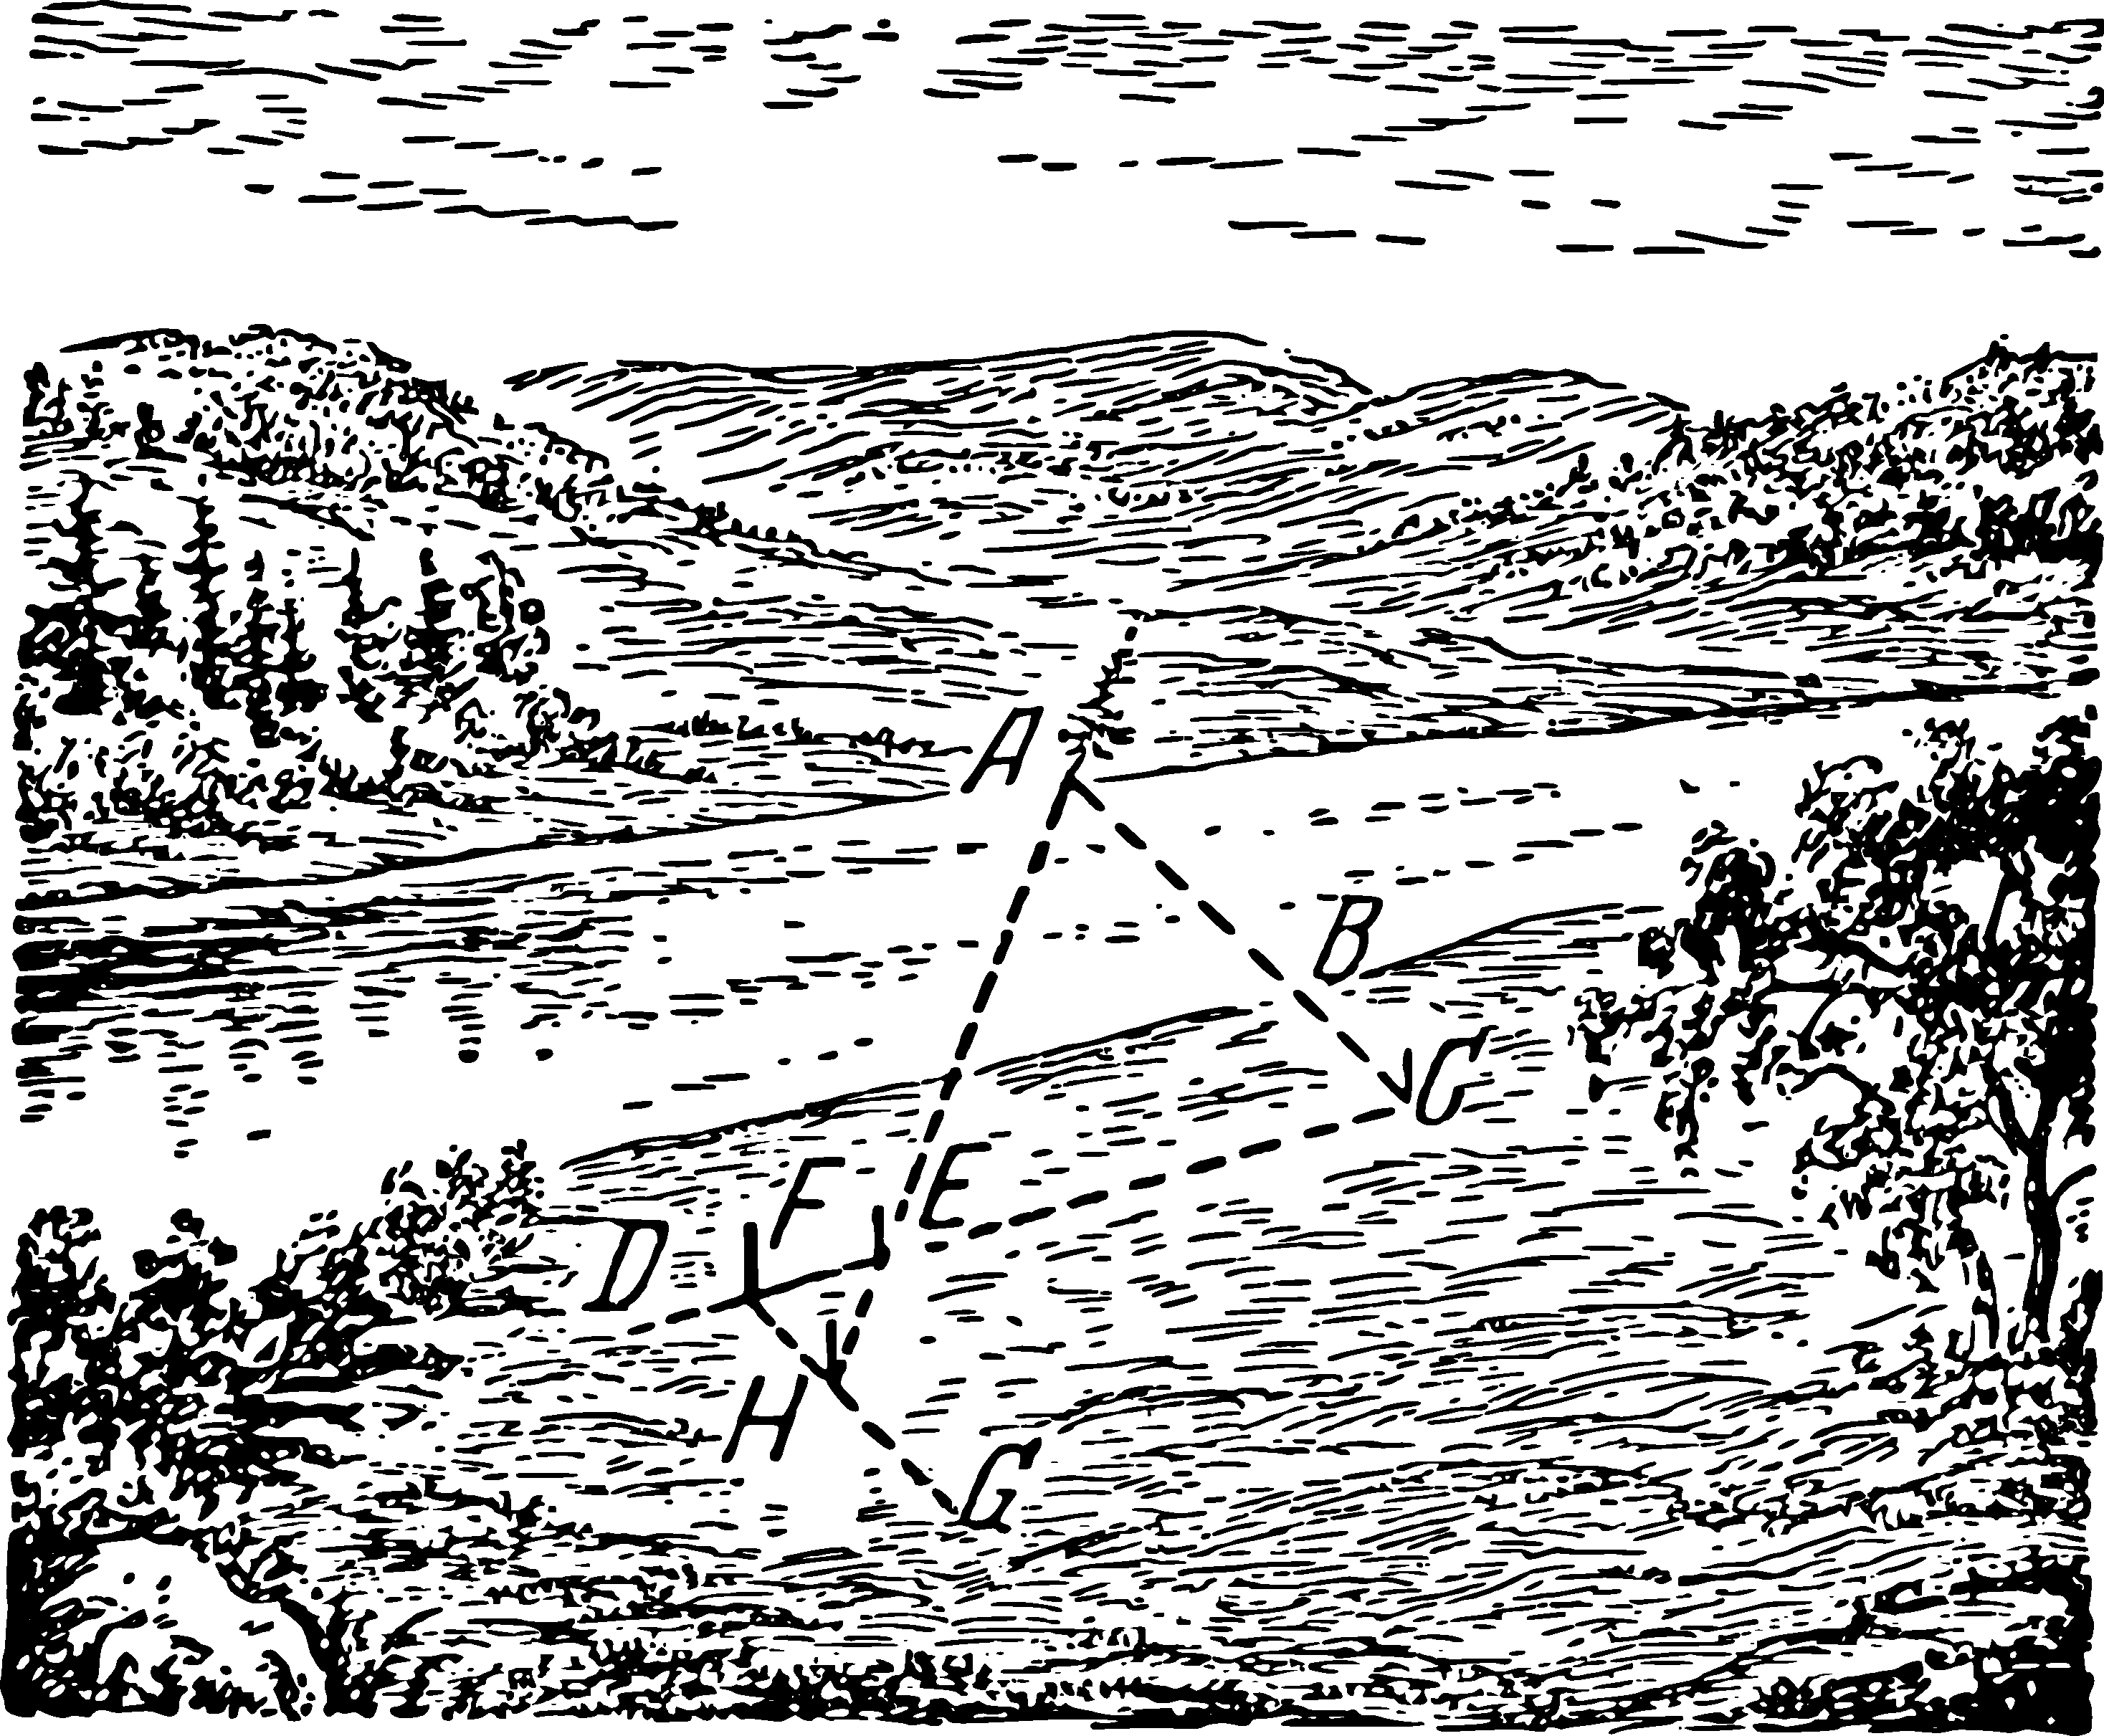
\includegraphics[width=0.9\textwidth]{figures/ch-02/fig-029.pdf}
\sidecaption{Using the similarity criteria of triangles to find the width of the river.\label{fig-029}}
\end{figure}

\item The method described above can be modified: instead of measuring equal distances on the straight line $CF$, measure one distance several times smaller than the other. For example (\figr{fig-029}), $FE$ is measured four times less than $EC$, and then we proceed as before: in the direction $FG$, perpendicular to $FC$, we find a point $H$ from which the peg $E$ appears to cover point $A$. But now $FH$ is no longer equal to $AC$, but four times smaller than this distance: triangles $ACE$ and $EFH$ are not congruent here, but similar (they have equal angles with unequal sides). From the similarity of triangles follows the proportion:
\begin{equation*}%
\frac{AC}{FH} = \frac{CE}{EF} = \frac{4}{1}
\end{equation*}
Therefore, by measuring $FH$ and multiplying the result by 4, we get the distance $AC$, and by subtracting $BC$, we find the desired width of the river.

This method, as we can see, requires less space and is therefore more convenient to perform than the previous one.




\item The fourth method is based on the property of a right triangle that if one of its acute angles is \ang{30}, then the length of the cathetus is half the hypotenuse. It is very easy to verify the correctness of this. 

Let angle $B$ of right triangle $ABC$ (\figr{fig-030}, left) be \ang{30}; we will prove that in this case, $AC = \nicefrac{1}{2}\, AB$. Rotate triangle $ABC$ around $BC$ so that it is symmetric with its initial position (\figr{fig-030}, right), forming figure $ABD$; line $AC$ is straight because both angles at point $C$ are right angles. In triangle $ABD$, angle $\angle A = \ang{60}$, angle $ABD$, composed of two \ang{30} angles, is also equal to \ang{60}. Therefore, $AD = BD$ as sides opposite equal angles. But $AC = \nicefrac{1}{2} \,AD$, therefore,
\begin{marginfigure}%[5cm]%[h!]
\centering
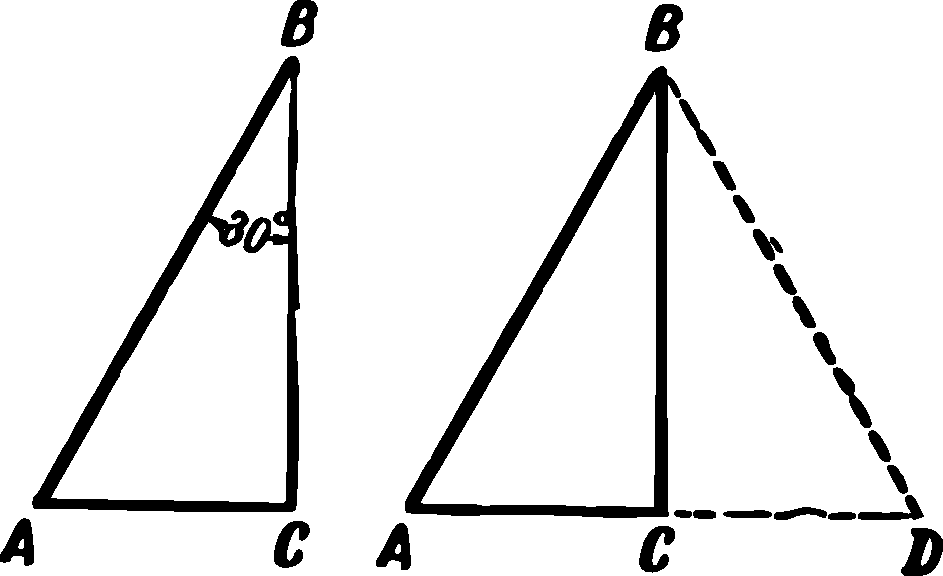
\includegraphics[width=\textwidth]{figures/ch-02/fig-030.pdf}
\sidecaption{When the cathetus is half the hypotenuse.\label{fig-030}}
\end{marginfigure}
\begin{equation*}%
AC = \frac{1}{2} AB.
\end{equation*}
Wishing to take advantage of this property of the triangle, we must arrange the pins on the board so that their bases represent a right triangle in which the cathetus is half the hypotenuse. With this device, we place ourselves at point $C$ (\figr{fig-031}) so that the direction $AC$ coincides with the hypotenuse of the pin triangle. 
\begin{marginfigure}%[5cm]%[h!]
\centering
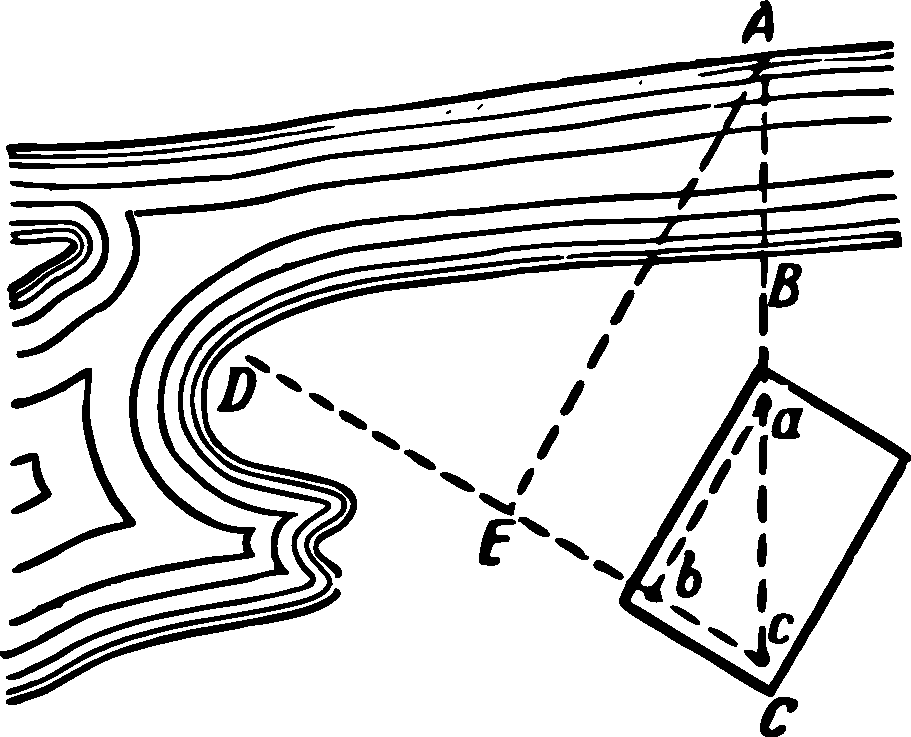
\includegraphics[width=\textwidth]{figures/ch-02/fig-031.pdf}
\sidecaption{The scheme of application of a right-angled triangle with a 30° angle.\label{fig-031}}
\end{marginfigure}
Looking along the short cathetus of this triangle, mark the direction $CD$ and find a point $E$ on it so that the direction $EA$ is perpendicular to $CD$ (this is done using the same pin device). It is easy to see that the distance $CE$ -- the cathetus lying opposite the angle of \ang{30} -- is equal to half of $AC$. Therefore, by measuring $CE$, doubling this distance and subtracting $BC$, we obtain the desired width of the $AB$ river.

\end{enumerate}

Here are four easily executable methods, with which it is always possible, without crossing to the other bank, to measure the width of the river with quite satisfactory accuracy. We will not consider methods that require the use of more complex instruments (even homemade ones) here.

\section{Using a visor}
\label{sec-2.2}

Here's how this method came in handy for Senior Sergeant Kupriyanov in frosty conditions.\sidenote{See the footnote on page~\pageref{ref-21}.} His detachment was ordered to measure the width of the river, across which they were to organise a crossing\ldots{}

Approaching a bush near the river, Kupriyanov's detachment took cover, and Kupriyanov himself, along with soldier Karpov, moved closer to the riverbank, from where the fascist-occupied shore was clearly visible. In such conditions, measuring the width of the river had to be done by eye.

``Come on, Karpov, how much?'' Kupriyanov asked.

``I think no more than 100-110 meters,'' Karpov replied. Kupriyanov agreed with his scout, but for control, he decided to measure the width of the river using a ``visor.''

\begin{figure}[h!]
\centering
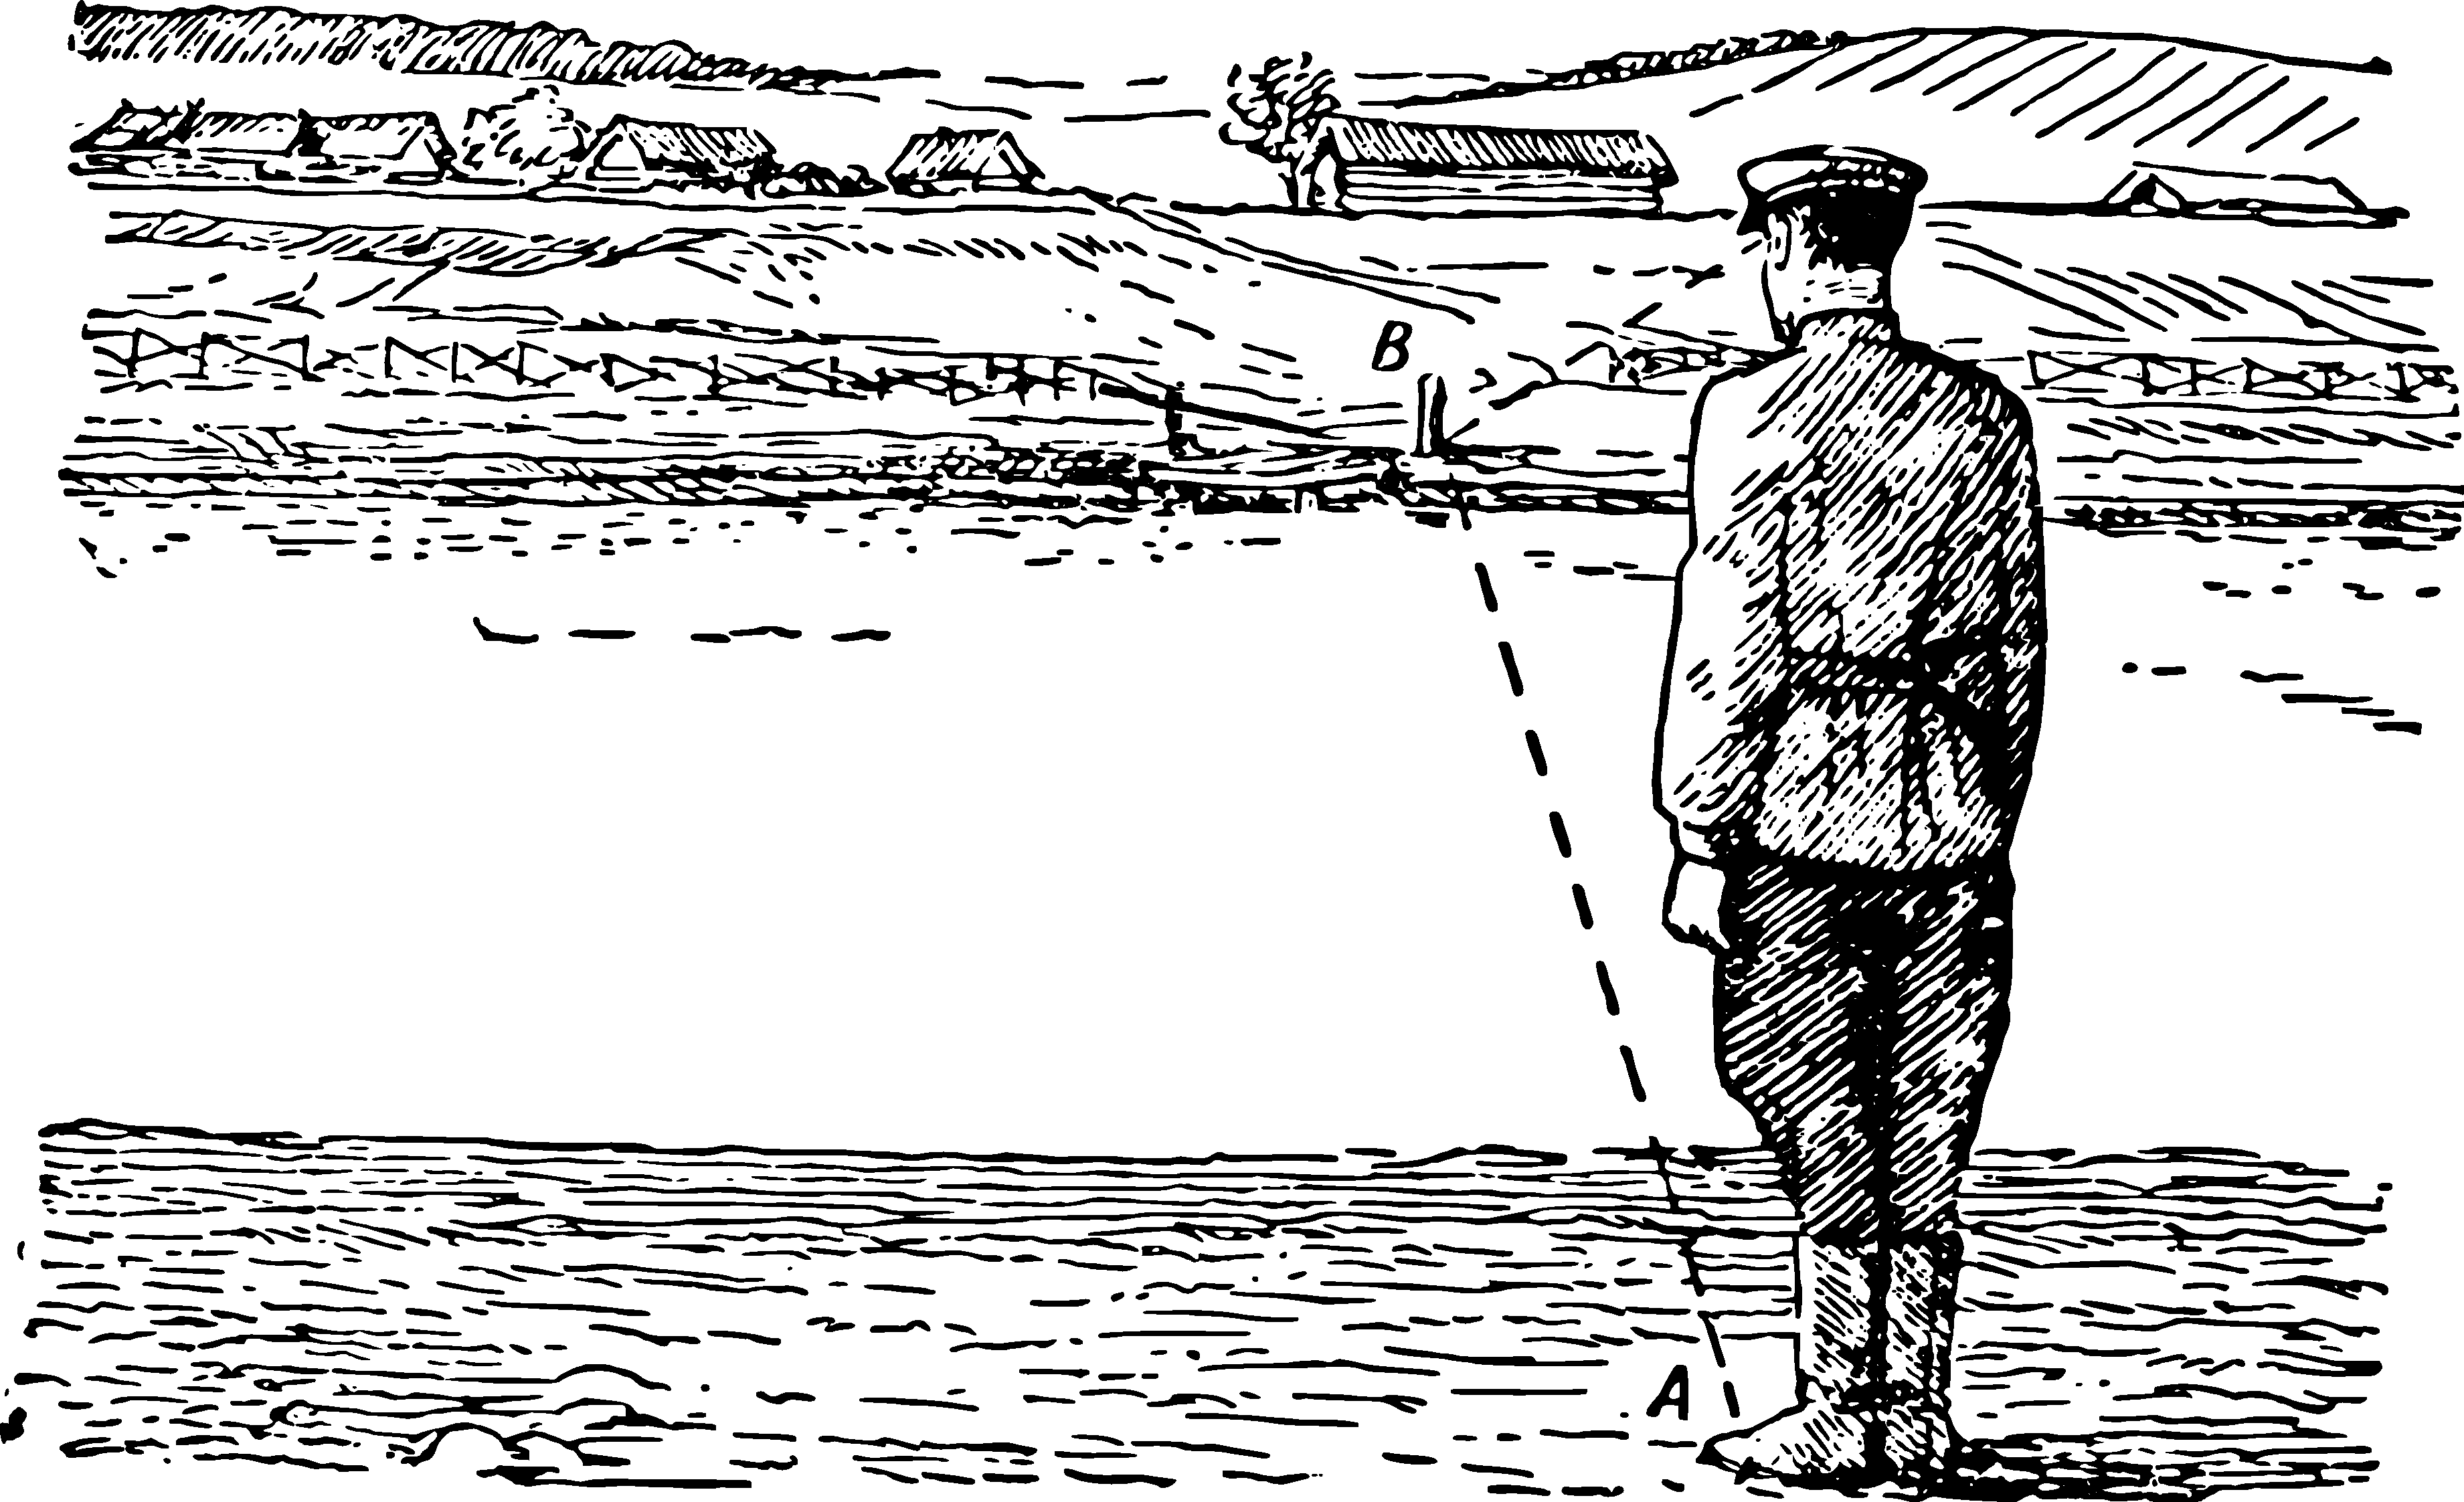
\includegraphics[width=0.9\textwidth]{figures/ch-02/fig-032.pdf}
\sidecaption{Observing a point on the opposite bank from under the visor.\label{fig-032}}
\end{figure}

This method is simple. You have to face the river and pull the visor over your eyes so that the lower edge of the visor precisely aligns with the line of the opposite bank (see \figr{fig-032}). The visor can be replaced with the palm of your hand or a notepad, tightly pressed edge to your forehead. Then, without changing the position of your head, you need to turn to the right or left, or even backward (towards the side where the area available for measuring the distance is more level) and notice the farthest point visible from under the visor (palm, notepad).

The distance to this point will be approximately equal to the width of the river.

Kupriyanov utilized this method. He quickly stood up in the bushes, pressed a notepad to his forehead, then quickly turned and aimed at the distant point. Then, together with Karpov, he crawled to that point, measuring the distance with a rope. It turned out to be 105 meters.

Kupriyanov reported the data he obtained to the command.

\ques Provide a geometric explanation for the ``visor'' method.

\begin{figure}[h!]
\centering
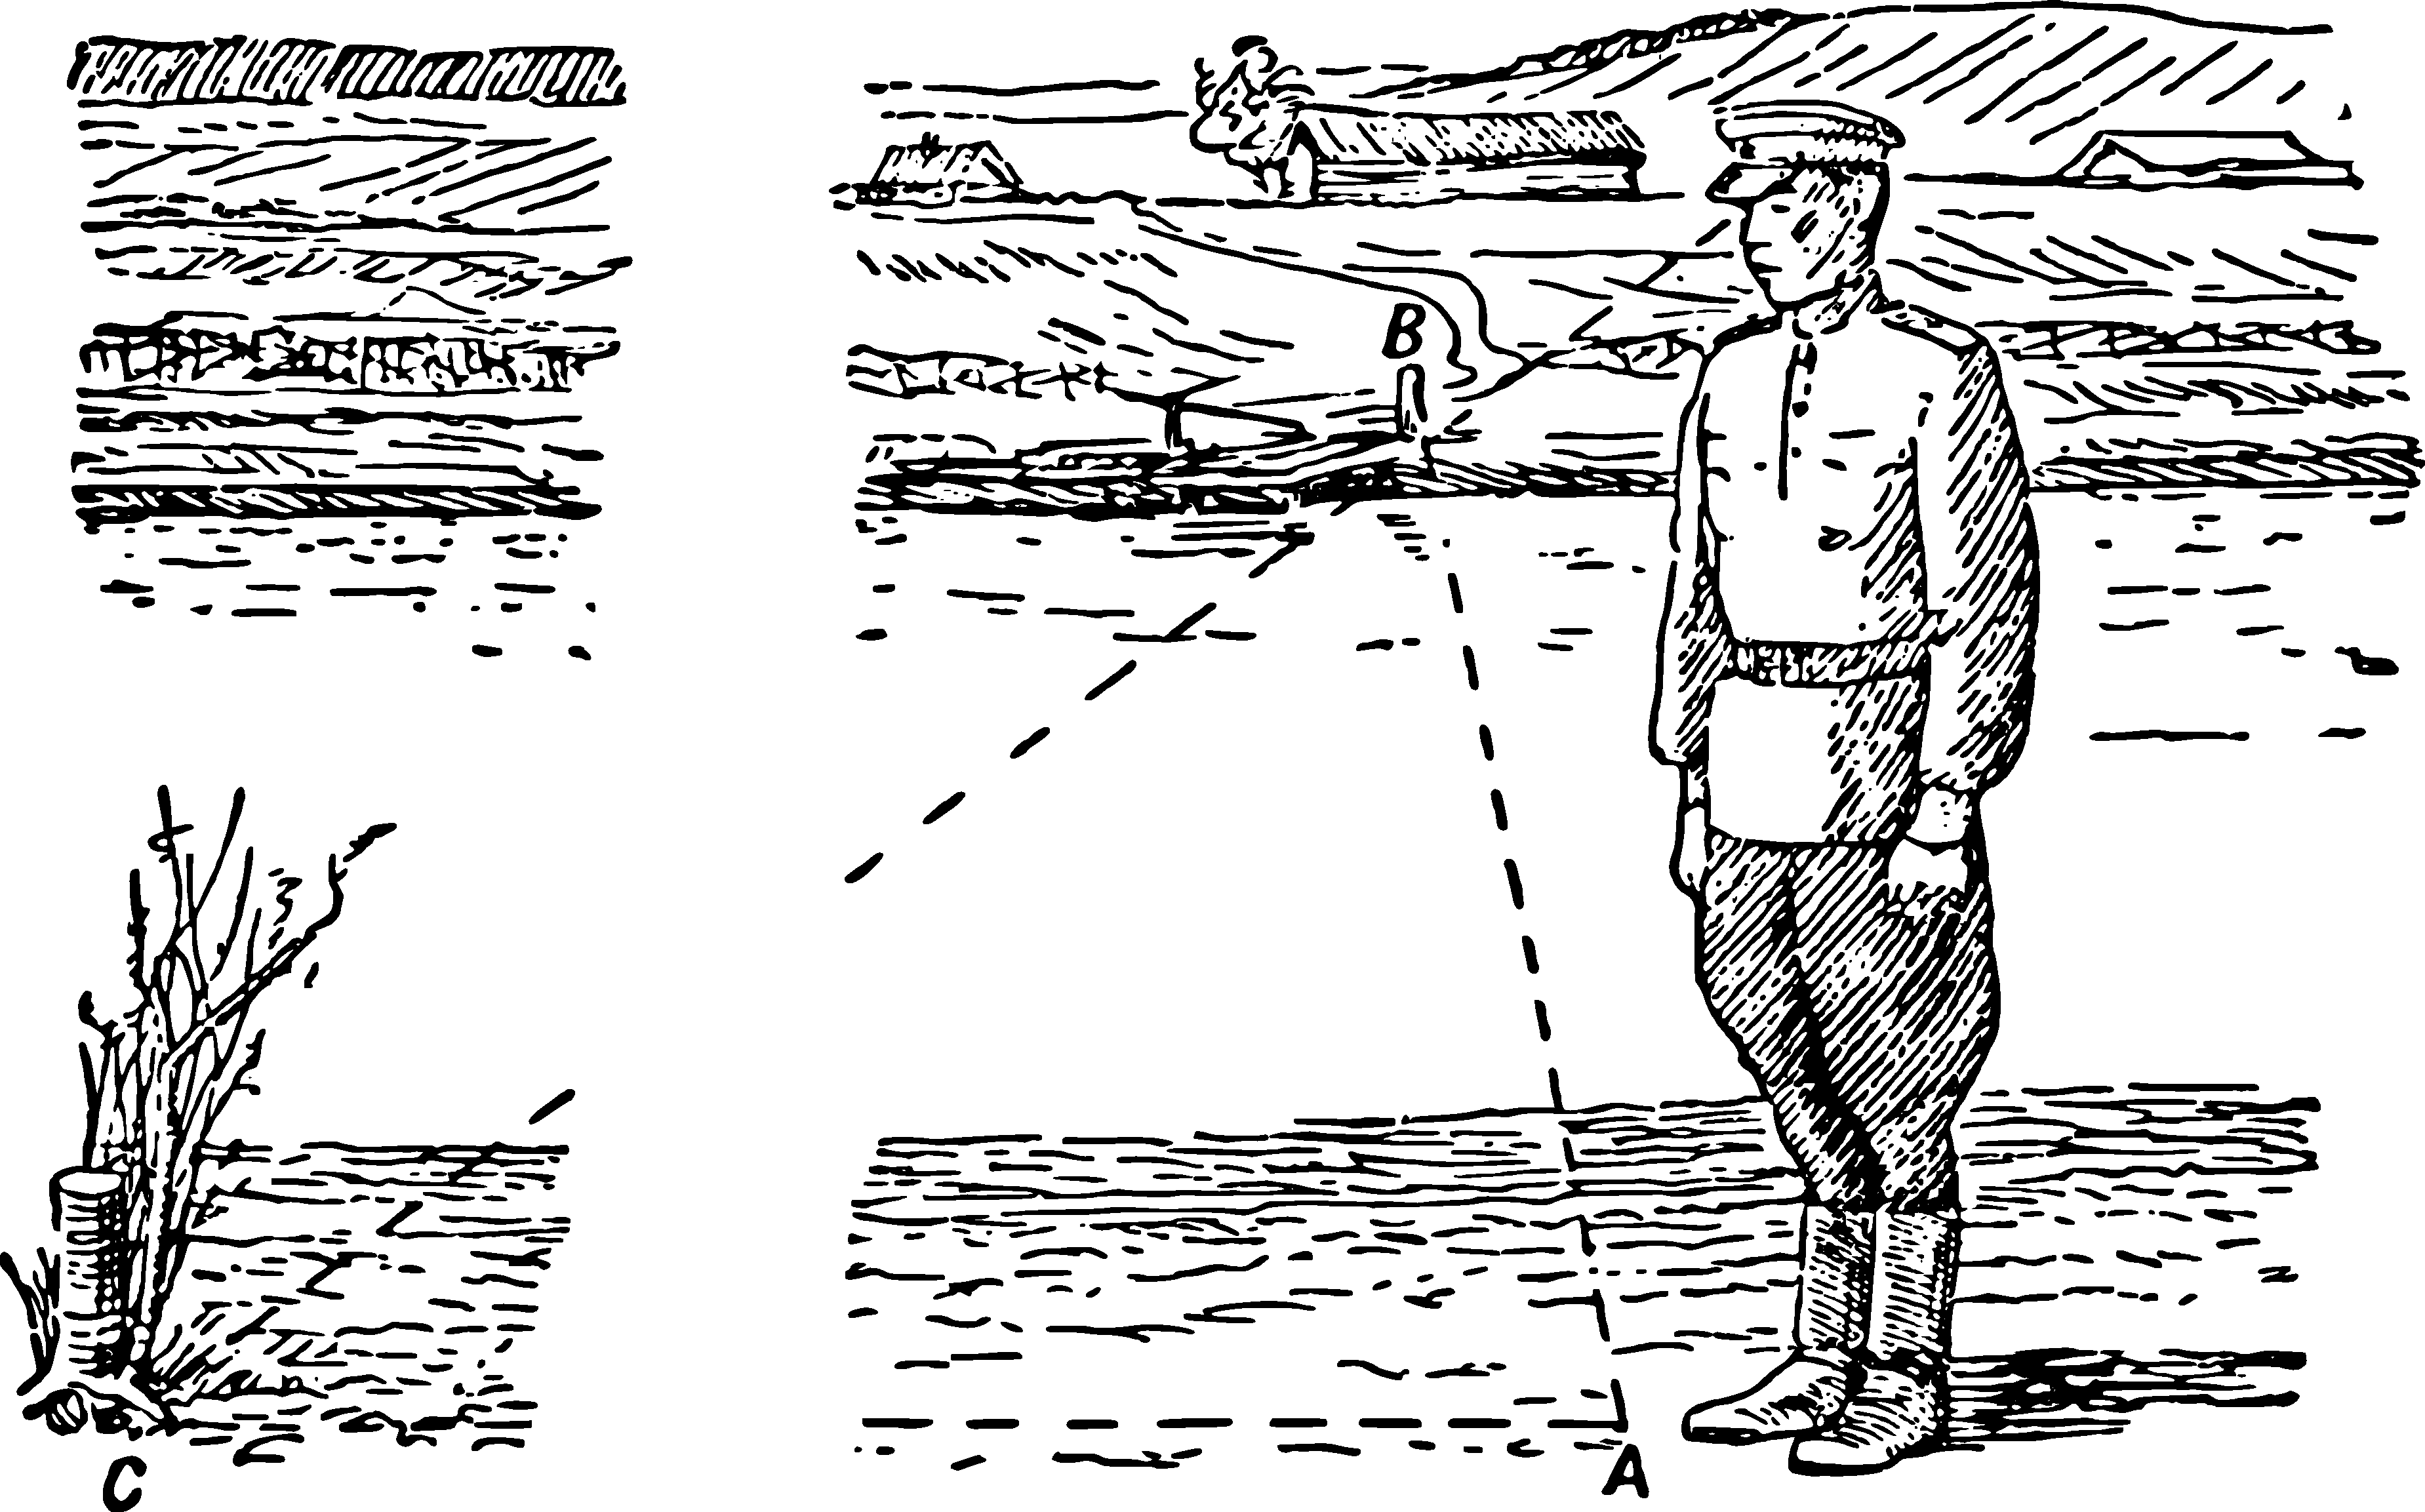
\includegraphics[width=0.9\textwidth]{figures/ch-02/fig-033.pdf}
\sidecaption{In the same way, you can aim at a point on your own bank.\label{fig-033}}
\end{figure}

\ans The line of sight, touching the edge of the visor (palm, notepad), is initially directed towards the line of the opposite bank (see \figr{fig-032}). When a person turns, the line of sight, like the leg of a compass, describes a circle, and then $AC = AB$ as the radii of the same circle (see \figr{fig-033}). 

\section{The Length Of An Island}

\ques Now we are faced with a more challenging task. Standing by the river or lake, you see an island (see \figr{fig-034}) whose length you wish to measure without leaving the shore. Is it possible to carry out such a measurement?

Although in this case, both ends of the measured line are inaccessible to us, the problem is still entirely solvable, and without complex instruments.

\begin{figure}[h!]
\centering
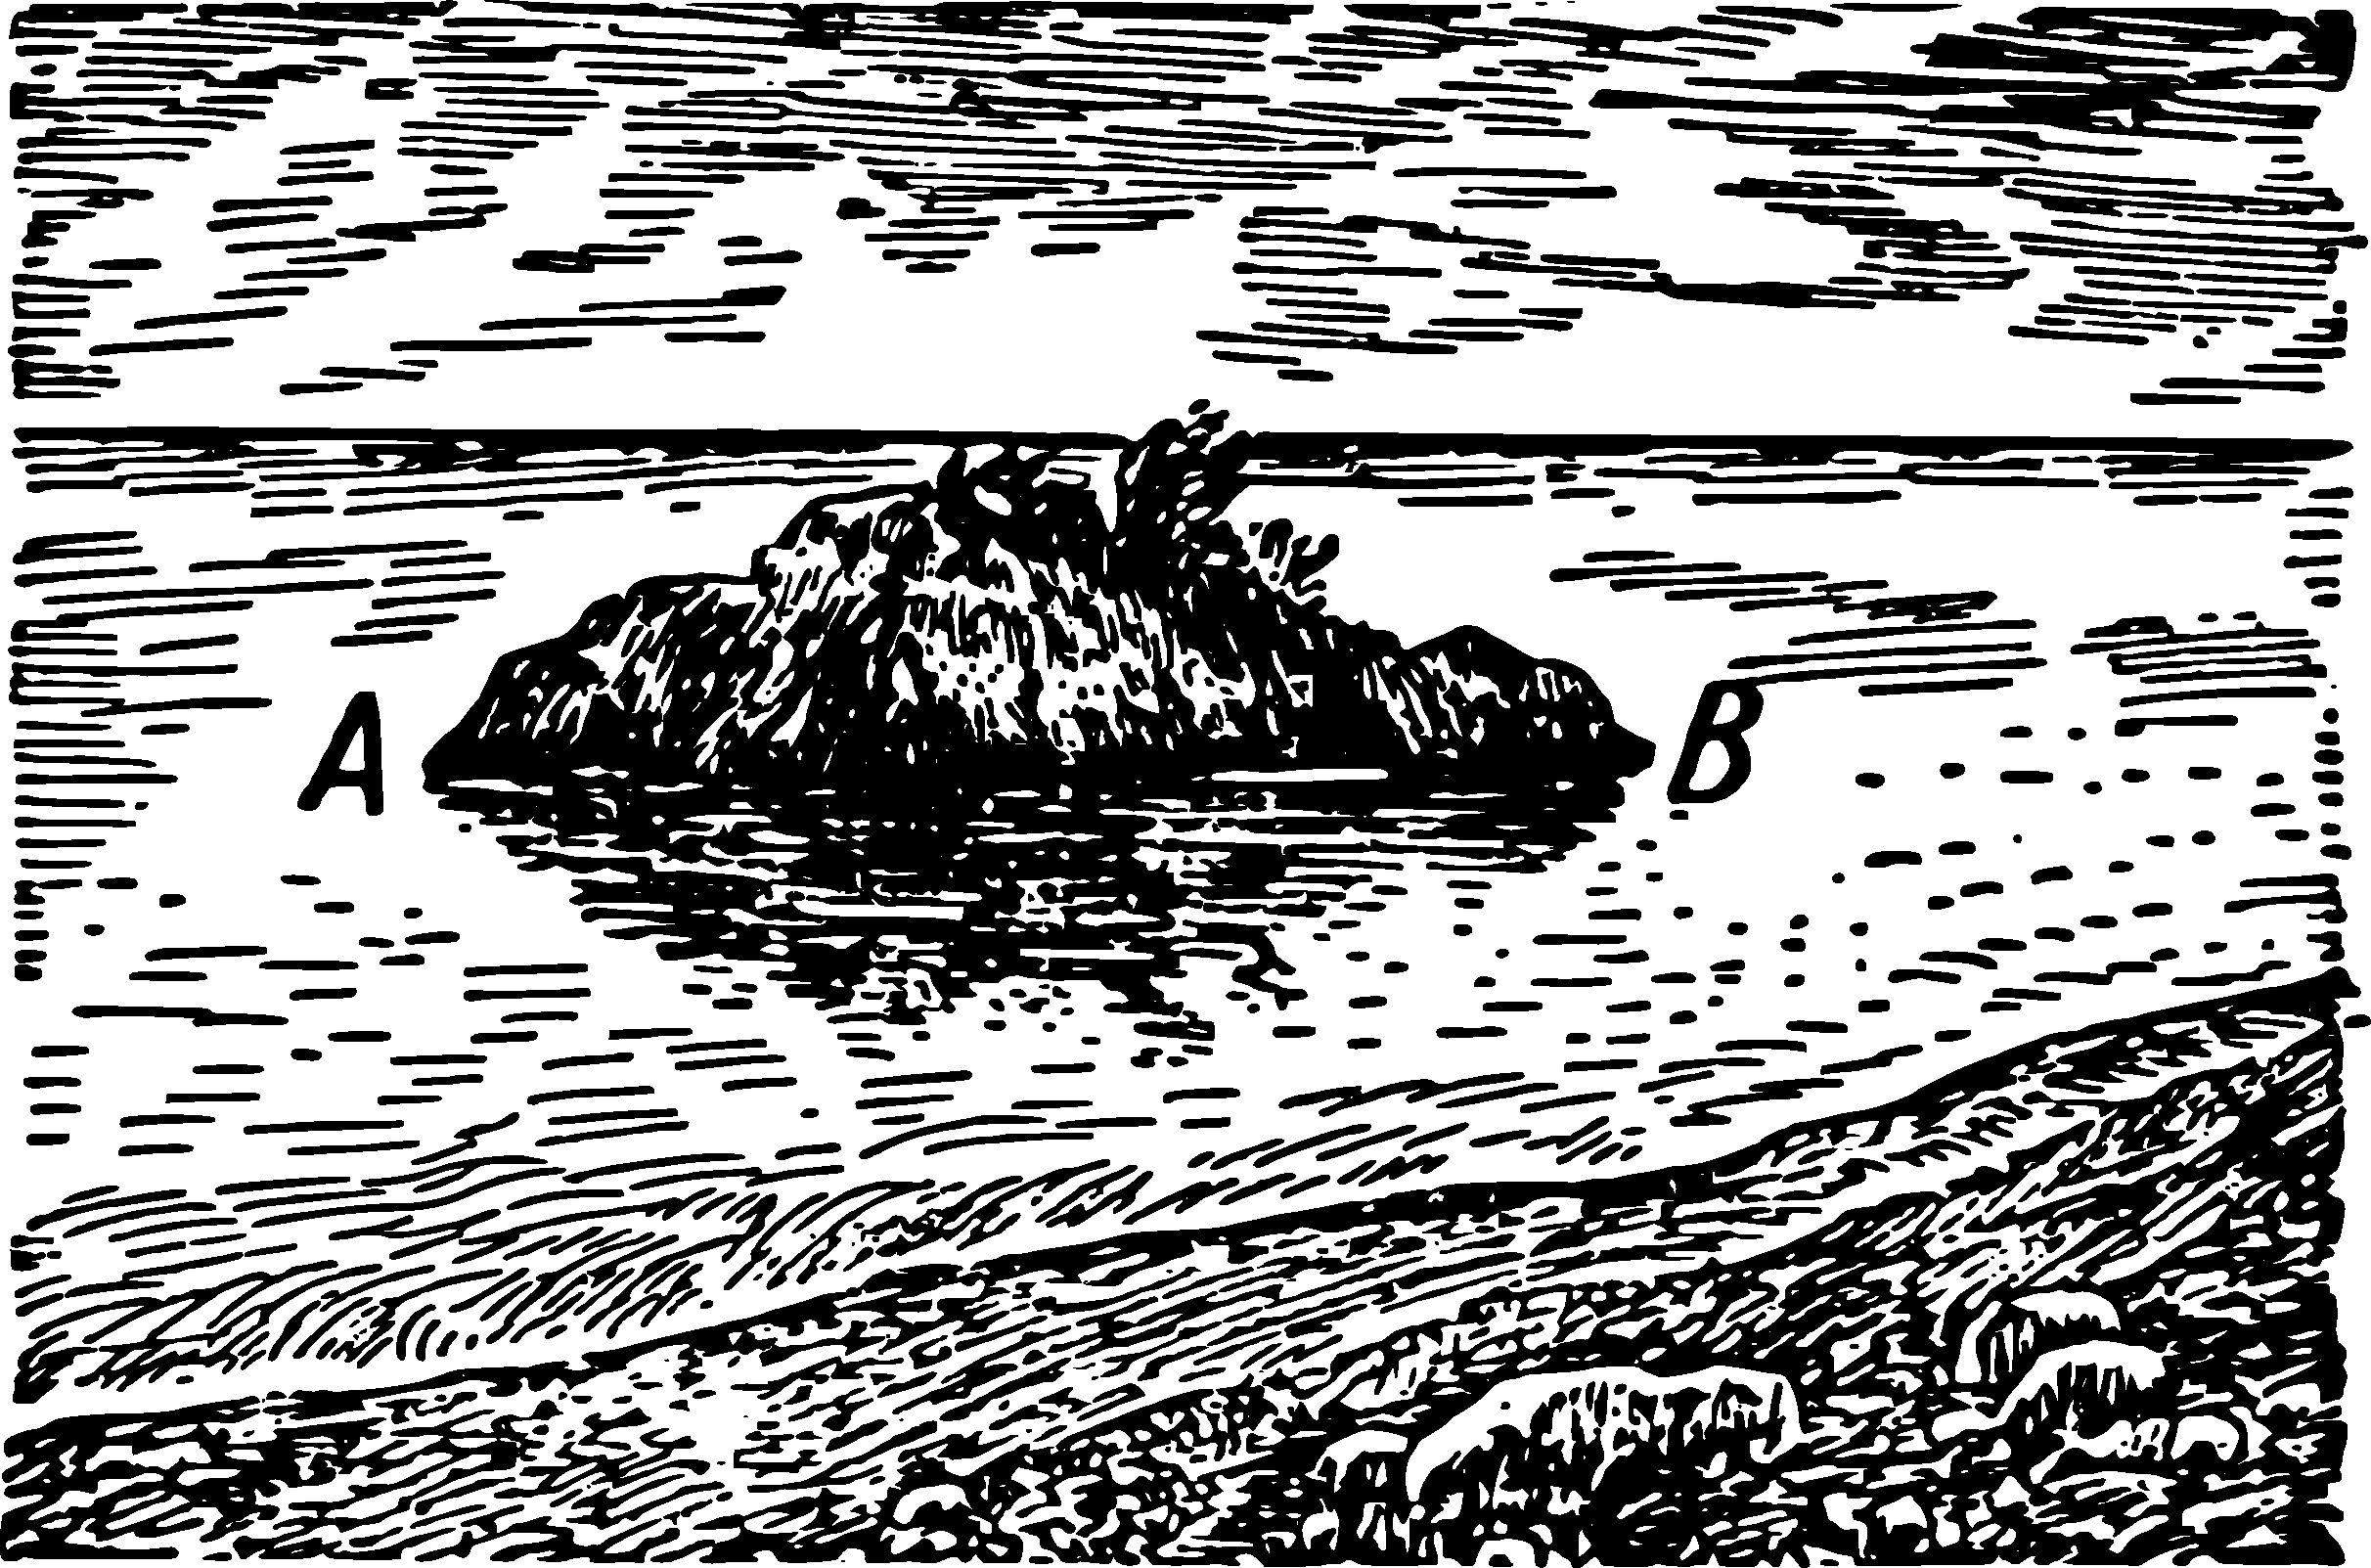
\includegraphics[width=0.9\textwidth]{figures/ch-02/fig-034.pdf}
\sidecaption{How to determine the length of the island.\label{fig-034}}
\end{figure}


\ans To measure the length of an island without leaving the shore, you can use the following method. Choose arbitrary points $P$ and $Q$ on the shore and place stakes in them. Then find points $M$ and $N$ on the line $PQ$ such that the directions $AM$ and $BM$ form right angles with the direction of $PQ$ (this can be done using a compass). In the middle of the distance $MN$, place a stake $O$ and find on the extension of the line $AM$ a point $C$ from which the stake $O$ appears to cover point $B$. Similarly, on the extension of $BN$, find point $D$ from which stake $O$ appears to cover the end $A$ of the island. The distance $CD$ will be the desired length of the island.

\begin{marginfigure}[-3cm]%[h!]
\centering
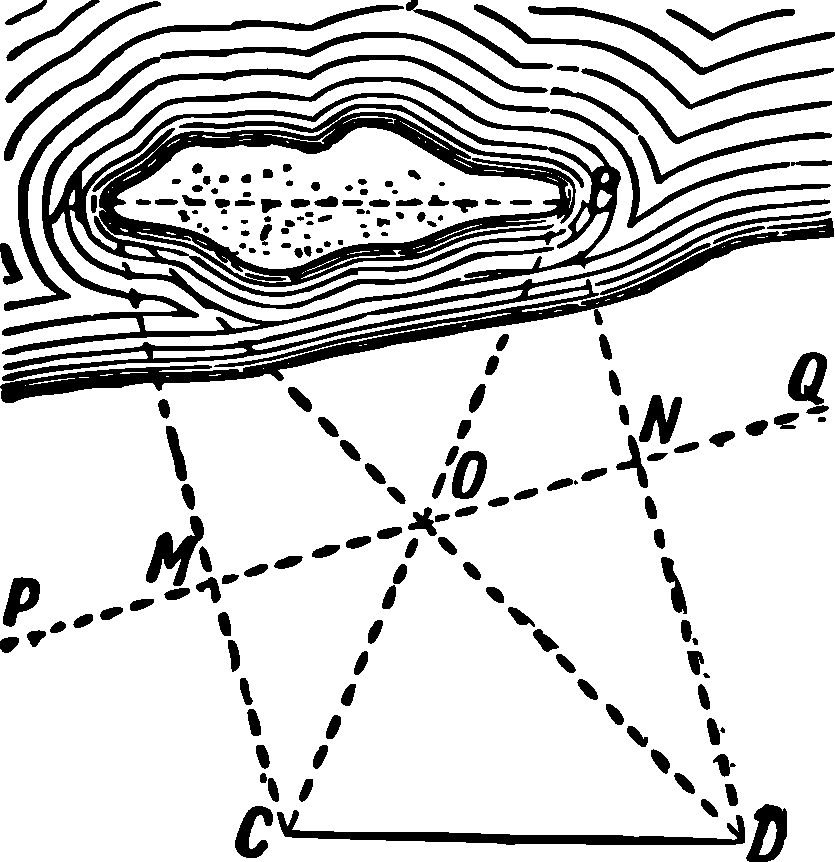
\includegraphics[width=\textwidth]{figures/ch-02/fig-035.pdf}
\sidecaption{We use the properties of congruent right triangles to find the length of an isalnd.\label{fig-035}}
\end{marginfigure}

This can be easily proved. Consider the right triangles $AMO$ and $OND$; in them, the legs $MO$ and $NO$ are equal, and the angles $AOM$ and $NOD$ are also equal, therefore, the triangles are equal, and $AO = OD$. Similarly, it can be proved that $BO = OC$. By comparing the triangles $ABO$ and $COD$, it can be seen that their distances $AB$ and $CD$ are equal.

\section{A pedestrian on the opposite bank}
\label{sec-2.3}

\ques As you walk along the riverbank, you see a person on the other side, and you can clearly distinguish their steps. Can you, without moving from your spot, determine at least approximately the distance between them and you? You have no instruments at hand.

\begin{figure}[h!]
\centering
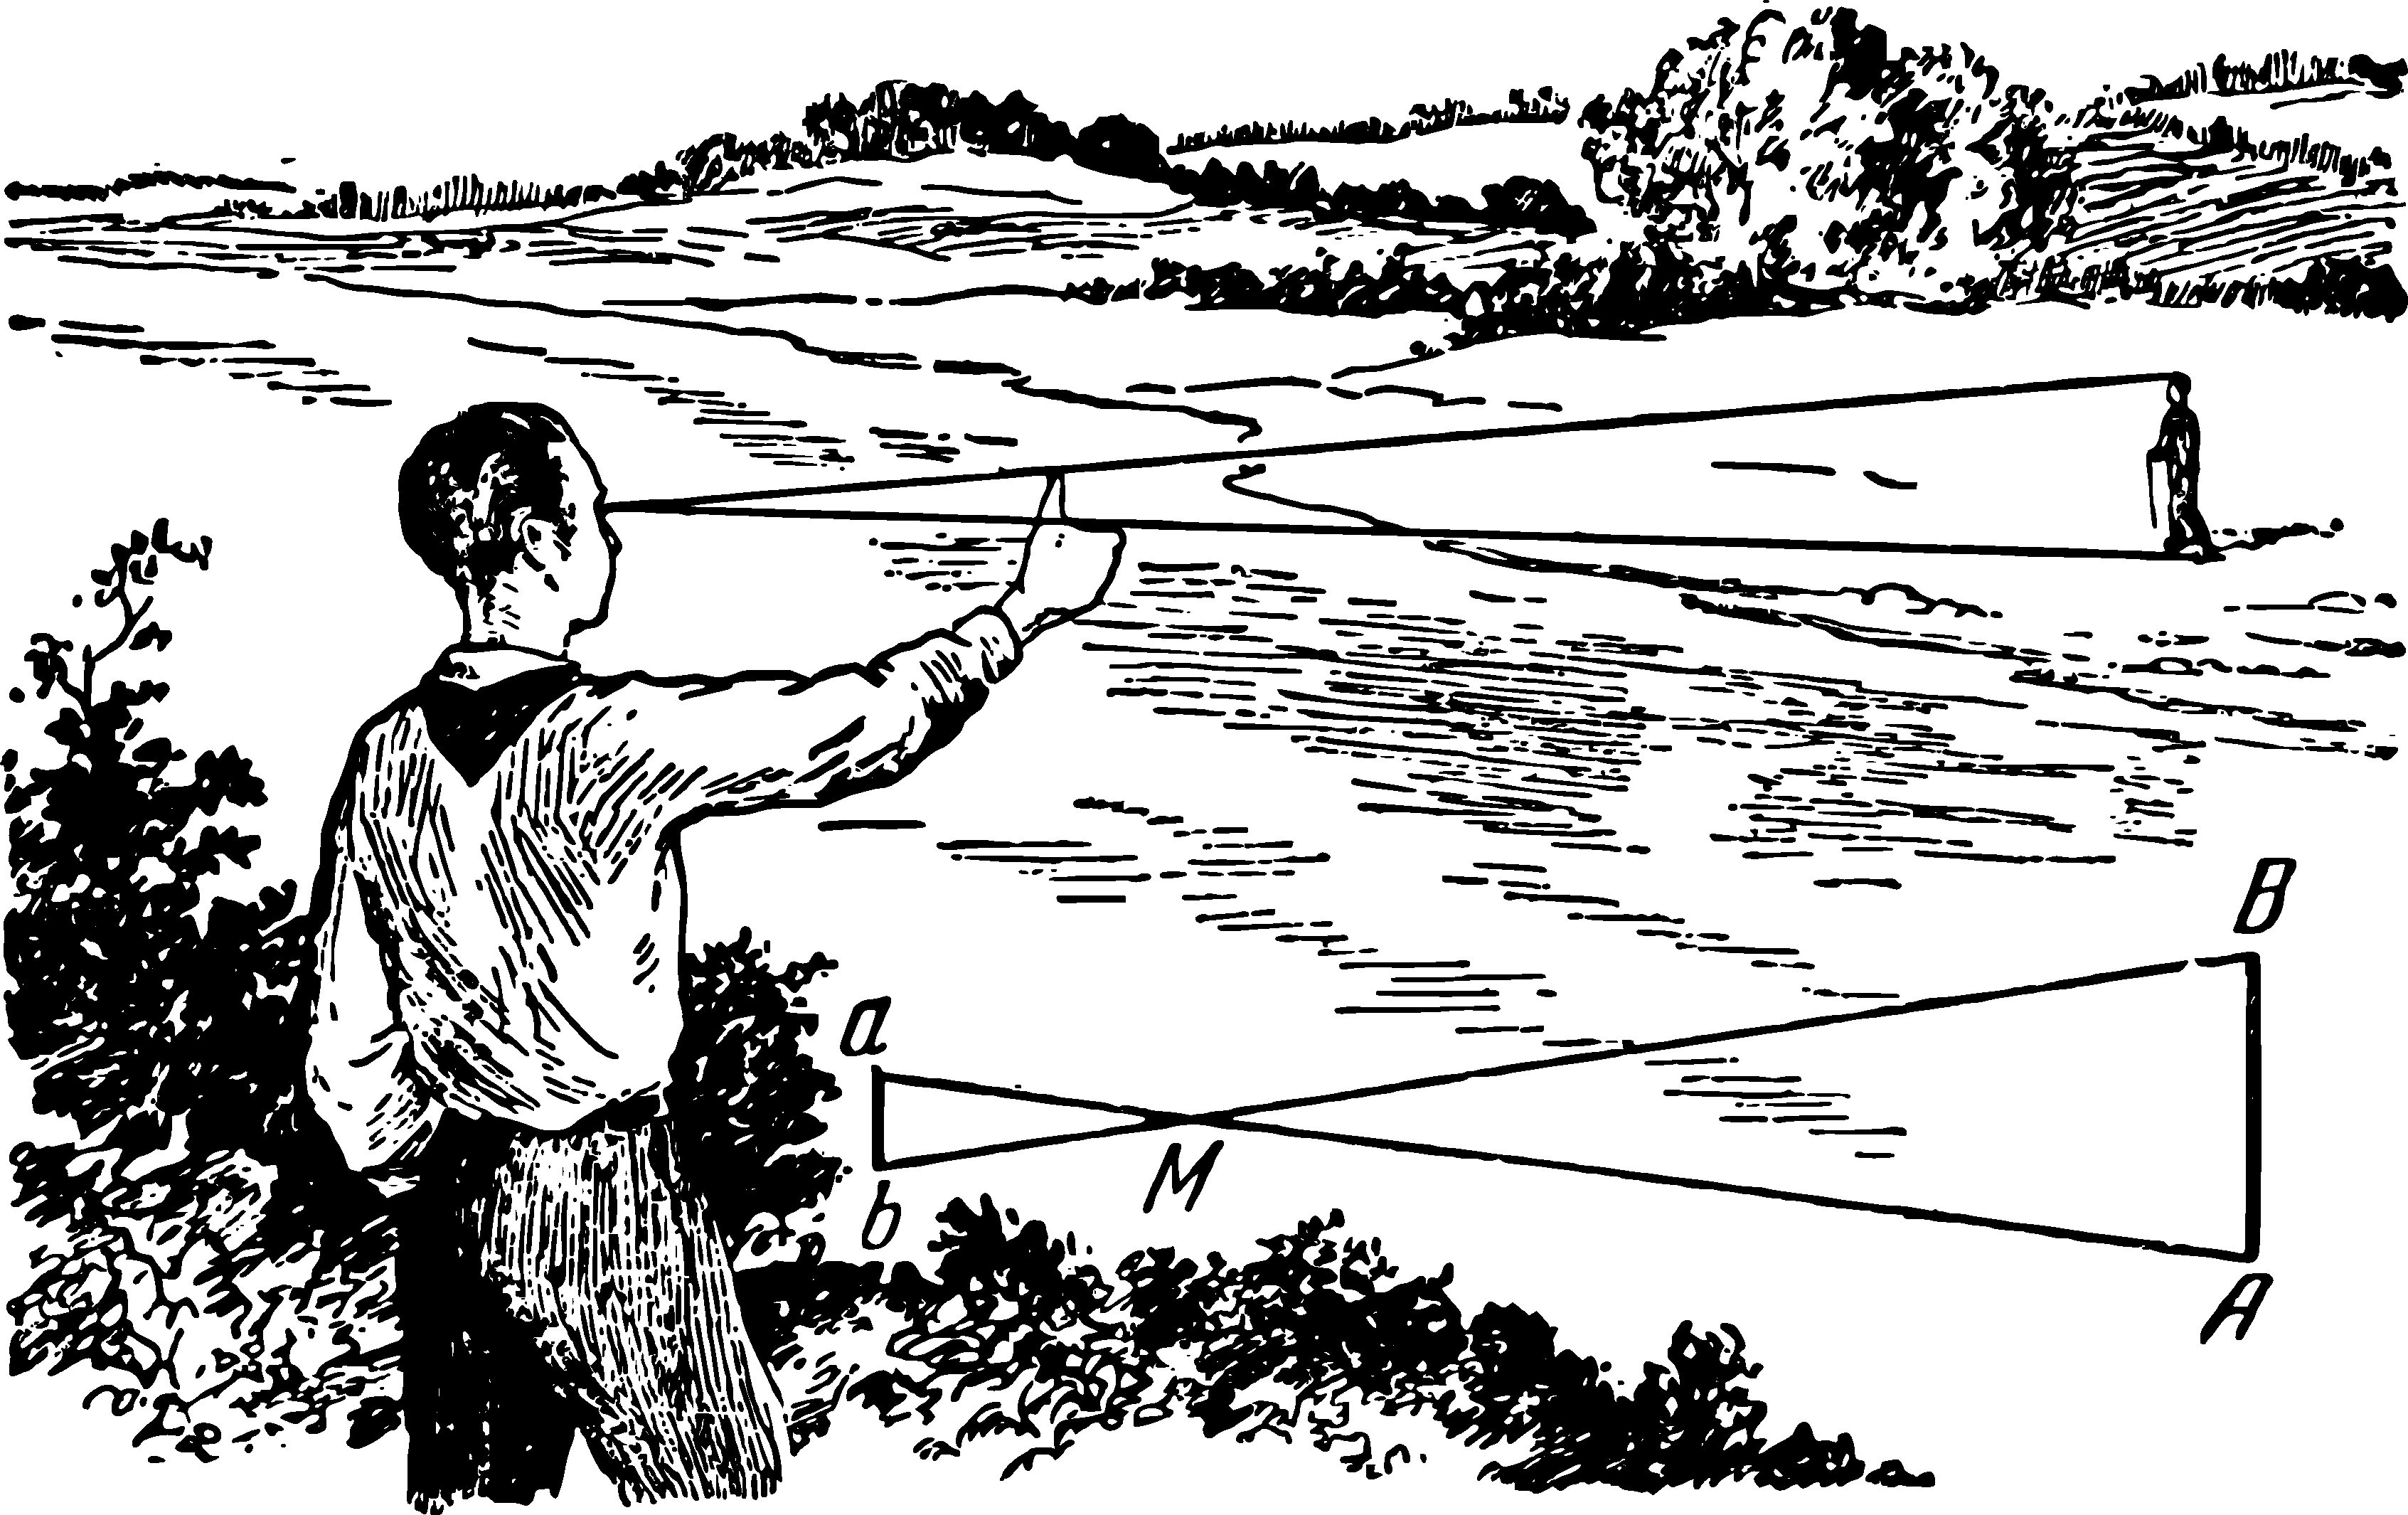
\includegraphics[width=0.9\textwidth]{figures/ch-02/fig-036.pdf}
\sidecaption{How to determine the distance to a pedestrian walking on the other side of the river.\label{fig-036}}
\end{figure}


\ans You don't have any instruments, but you have eyes and hands -- that's enough. Extend your arm forward towards the pedestrian and look at the tip of your finger with one eye if the pedestrian is moving towards your right hand, and with the other eye if they're moving towards your left hand. At the moment when the distant pedestrian is covered by your finger (see \figr{fig-036}), close the eye that was looking and open the other: the pedestrian will appear to you as if they've moved backward. Count how many steps they take before they align again with your finger. You'll get all the data needed for an approximate determination of the distance. Let's explain how to use them.

Suppose in \figr{fig-036} (inset), your eyes are marked as $a$ and $b$, point $M$ is the tip of your finger extended, point $A$ is the initial position of the pedestrian, and $B$ is the final position. The triangles $abM$ and $ABM$ are similar (you should turn towards the pedestrian so that $ab$ is approximately parallel to their direction of movement). Therefore, $BM : bM = AB : ab$ -- is a proportion in which only one term, $BM$, is unknown, but all others can be directly determined. Indeed, $bM$ is the length of your extended arm, $ab$ is the distance between the pupils of your eyes, and $AB$ is measured in steps taken by the pedestrian (assuming an average step to be around 3/4 metres). Therefore, the unknown distance from you to the pedestrian on the opposite bank, $AB$, equals 
\begin{equation*}%
MB = AB \, \frac{bM}{ab}
\end{equation*}
For example, if the distance between your eye pupils $ab$ is \SI{6}{\centi\meter}, the length of $bM$ from the end of your extended arm to the eye is \SI{60}{\centi\meter}, and the pedestrian takes, say, 14 steps from $A$ to $B$, then their distance from you would be $MB = 14 \cdot 60/6 = 140$ steps, or 105 meters.

It's enough for you to measure in advance the distance between your eye pupils and $bM$ -- the distance from the eye to the end of your extended arm -- so that you can quickly determine the distance of inaccessible objects by remembering their ratio. On average, for most people, $bM/ab$ is around 10 with slight fluctuations. The difficulty will only be in somehow determining the distance $AB$. In our case, we used the steps of a distant person. But you can also use other references. For instance, if you're measuring the distance to a distant freight train, you can estimate $AB$ in comparison to the length of a freight car, which is usually known (7.6 meters between buffers). If you're determining the distance to a house, you can estimate $AB$ by comparing it to the width of a window, the length of a brick, etc.

The same method can be applied to determine the size of a distant object if its distance from the observer is known. For this purpose, you can also use other ``rangefinders'', which we will describe next.

\section{Simple Rangefinders}
\begin{marginfigure}[-2cm]%[h!]
\centering
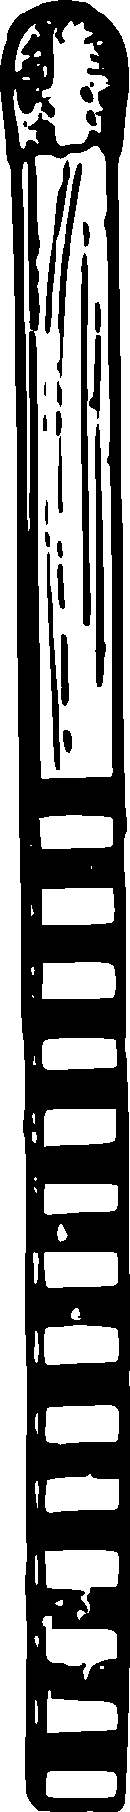
\includegraphics[width=0.1\textwidth]{figures/ch-02/fig-037.pdf}
\sidecaption{The match is a rangefinder.\label{fig-037}}
\end{marginfigure}
In the first chapter, we described the simplest instrument for determining inaccessible heights -- the altimeter. Now, let's describe the simplest device for measuring inaccessible distances -- the `rangefinder.' The simplest rangefinder can be made from an ordinary matchstick. To do this, you just need to mark millimeter divisions on one of its sides, alternating between light and dark (see \figr{fig-037}).


You can use this primitive ``rangefinder'' to estimate the distance to a distant object only in those cases when the dimensions of that object are known to you (see \figr{fig-038}). However, more sophisticated rangefinders can also be used under the same condition. Suppose you see a person in the distance and set yourself the task of determining the distance to them. Here, the matchstick rangefinder can come in handy. Holding it in your outstretched arm and looking with one eye, you bring its free end into coincidence with the top of the distant figure. Then, slowly moving your thumbnail along the matchstick, you stop it at the point that projects onto the base of the human figure. All you have to do now is to find out, by bringing the matchstick closer to the eye, at which mark your thumbnail stopped -- and then you have all the data to solve the problem.

\begin{figure}[h!]
\centering
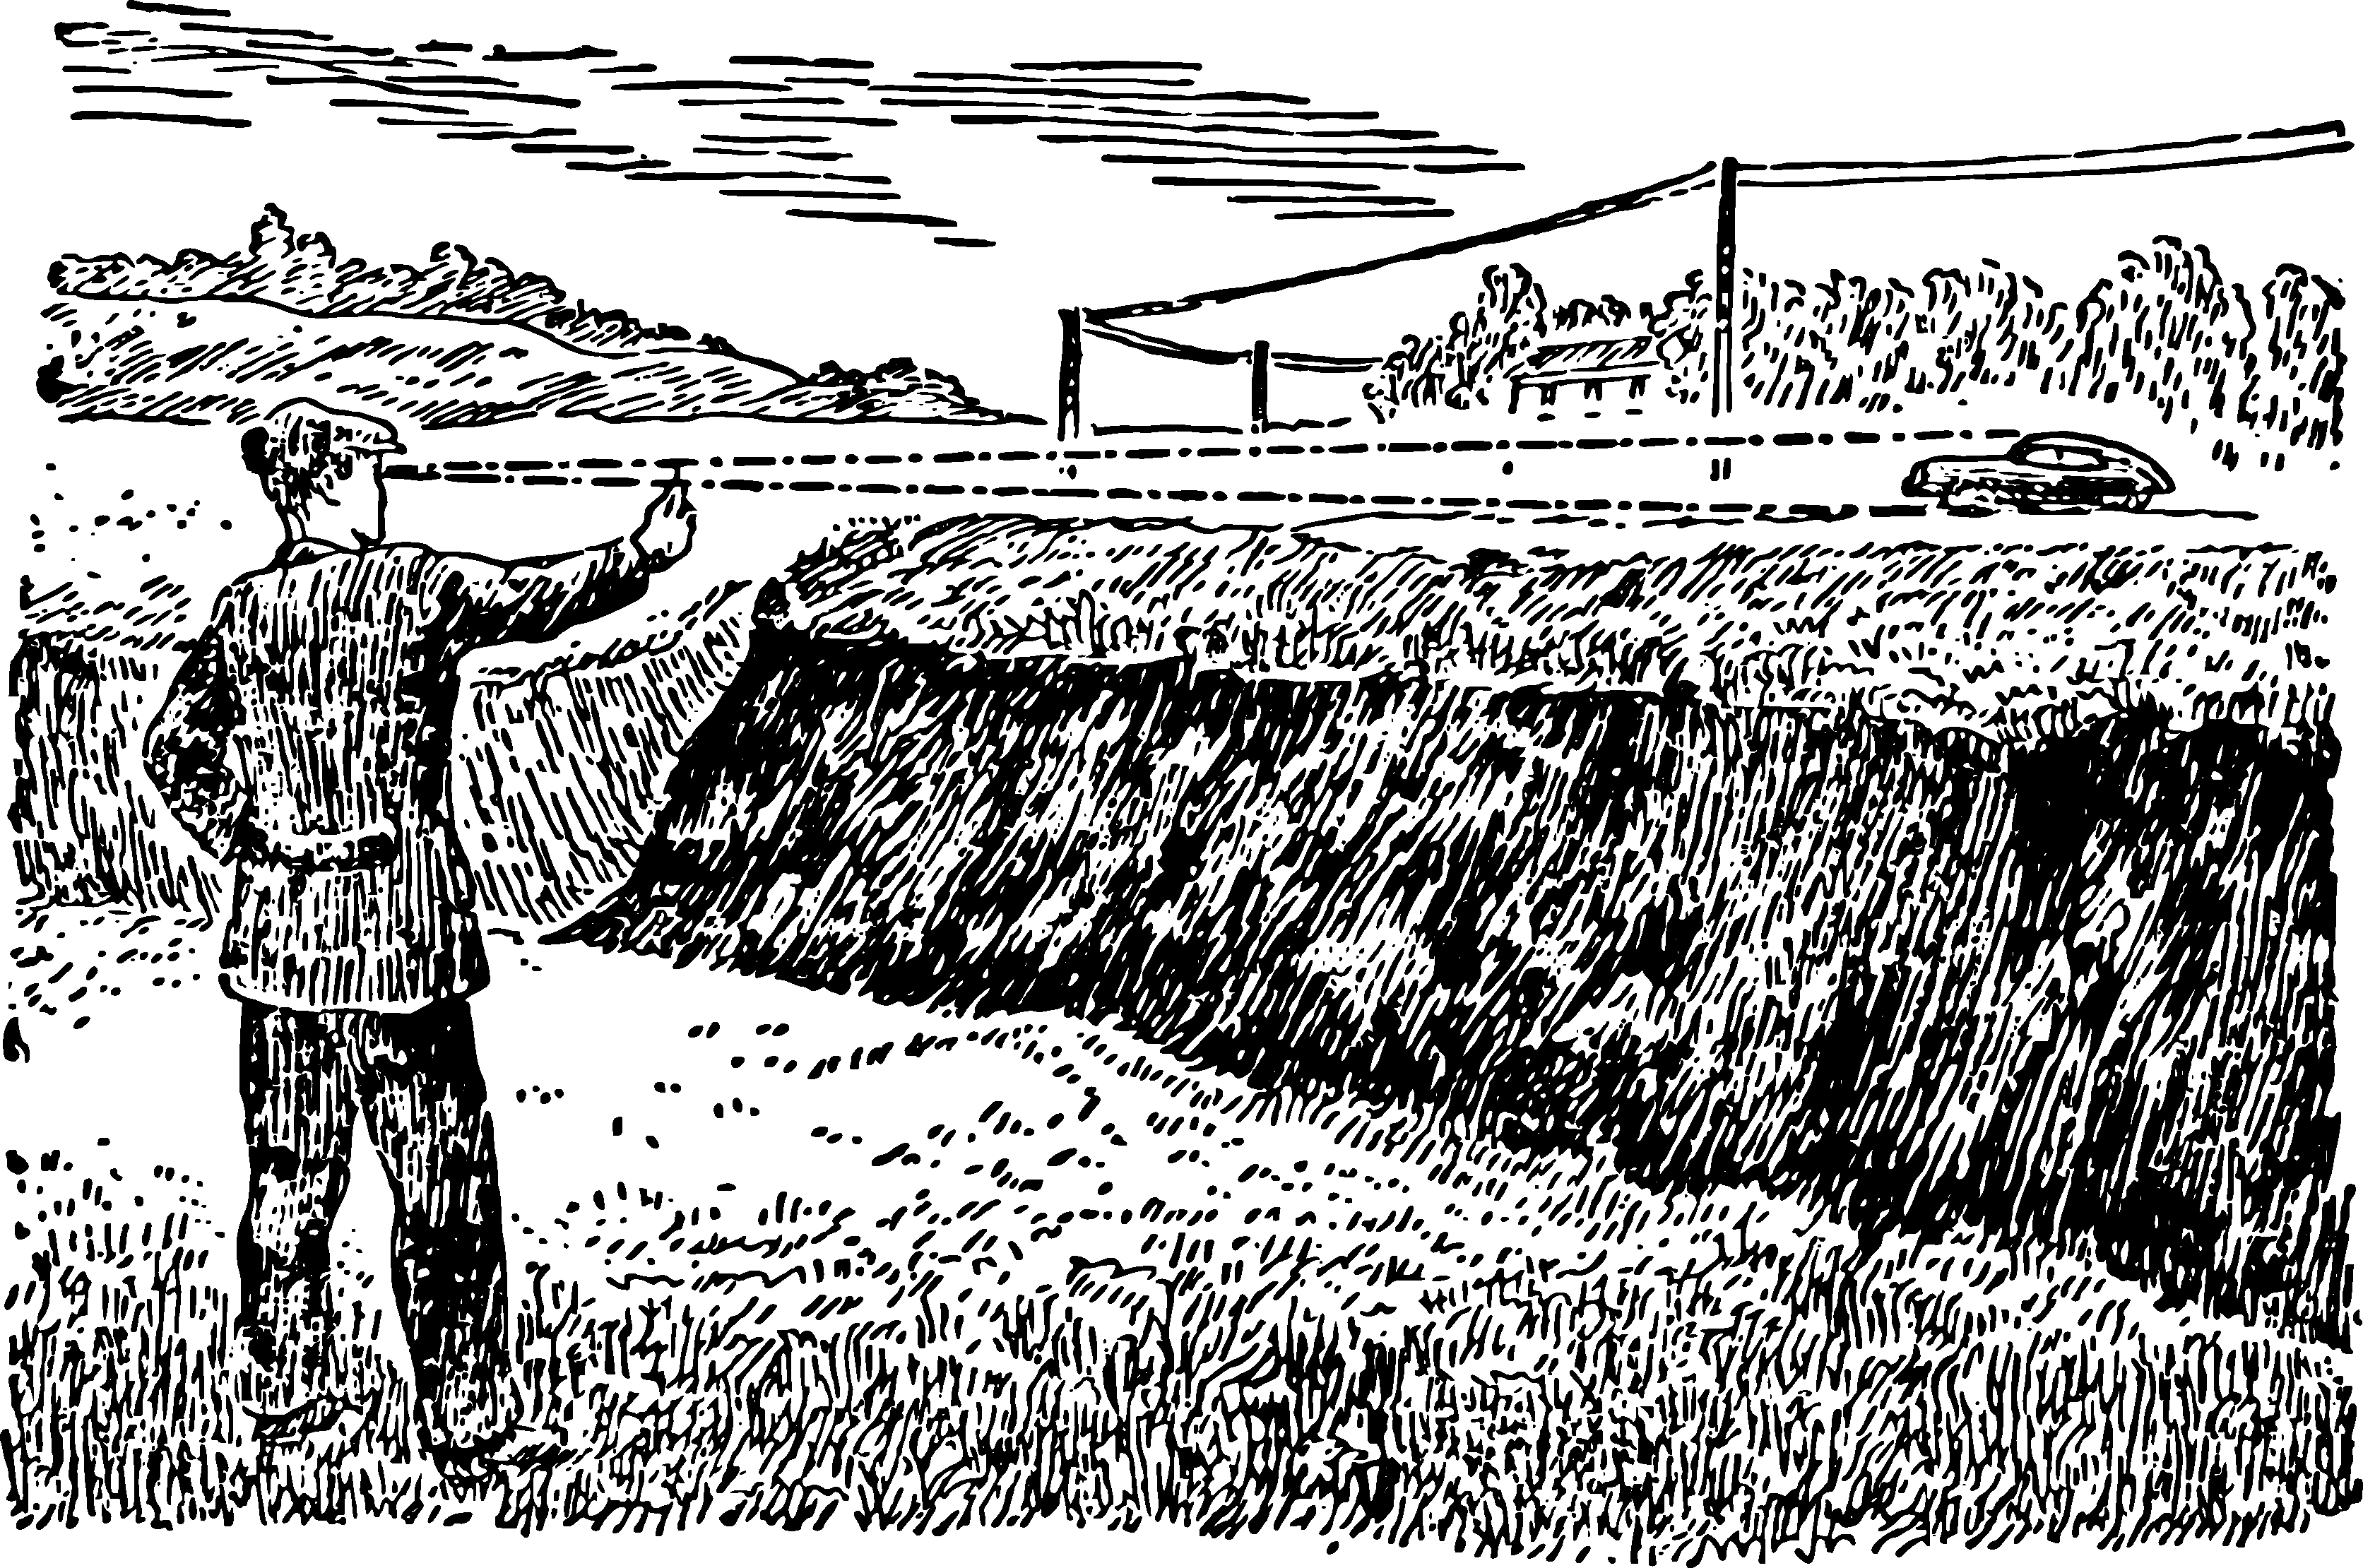
\includegraphics[width=\textwidth]{figures/ch-02/fig-038.pdf}
\sidecaption{The use of a rangefinder match to determine inaccessible distances.\label{fig-038}}
\end{figure}

You can easily verify the correctness of the proportion:
\begin{equation*}%
\frac{\text{desired distance}}{\begin{array}{c}\text{distance from the eye}\\ \text{to the matchstick}\end{array}} = \frac{\text{average height of a person}}{\begin{array}{c}\text{measured part}\\ \text{of the matchstick}\end{array}}
\end{equation*}
From here, it's easy to calculate the desired distance. For example, if the distance to the matchstick is \SI{60}{\centi\meter}, the height of the person is \SI{1.7}{\meter}, and the measured part of the matchstick is \SI{12}{\milli\meter}, then the determined distance would be:
\begin{equation*}%
60 \cdot \frac{1700}{12} = \SI{8500}{\centi\meter} = \SI{85}{\meter}.
\end{equation*}
To gain some skill in using this rangefinder, measure the height of someone from your group and, asking them to move away a certain distance, try to determine how many steps they took away from you.

With the same method, you can determine the distance to a rider (average height \SI{2.2}{\meter}), a cyclist (wheel diameter \SI{75}{\centi\meter}), a telegraph pole along the railway track (height \SI{8}{\meter}), vertical distance between adjacent insulators (\SI{90}{\centi\meter}), to a train, a brick house, and similar objects whose dimensions can be estimated with sufficient accuracy. There can be quite a few such cases during excursions.

\begin{marginfigure}%[-2cm]%[h!]
\centering
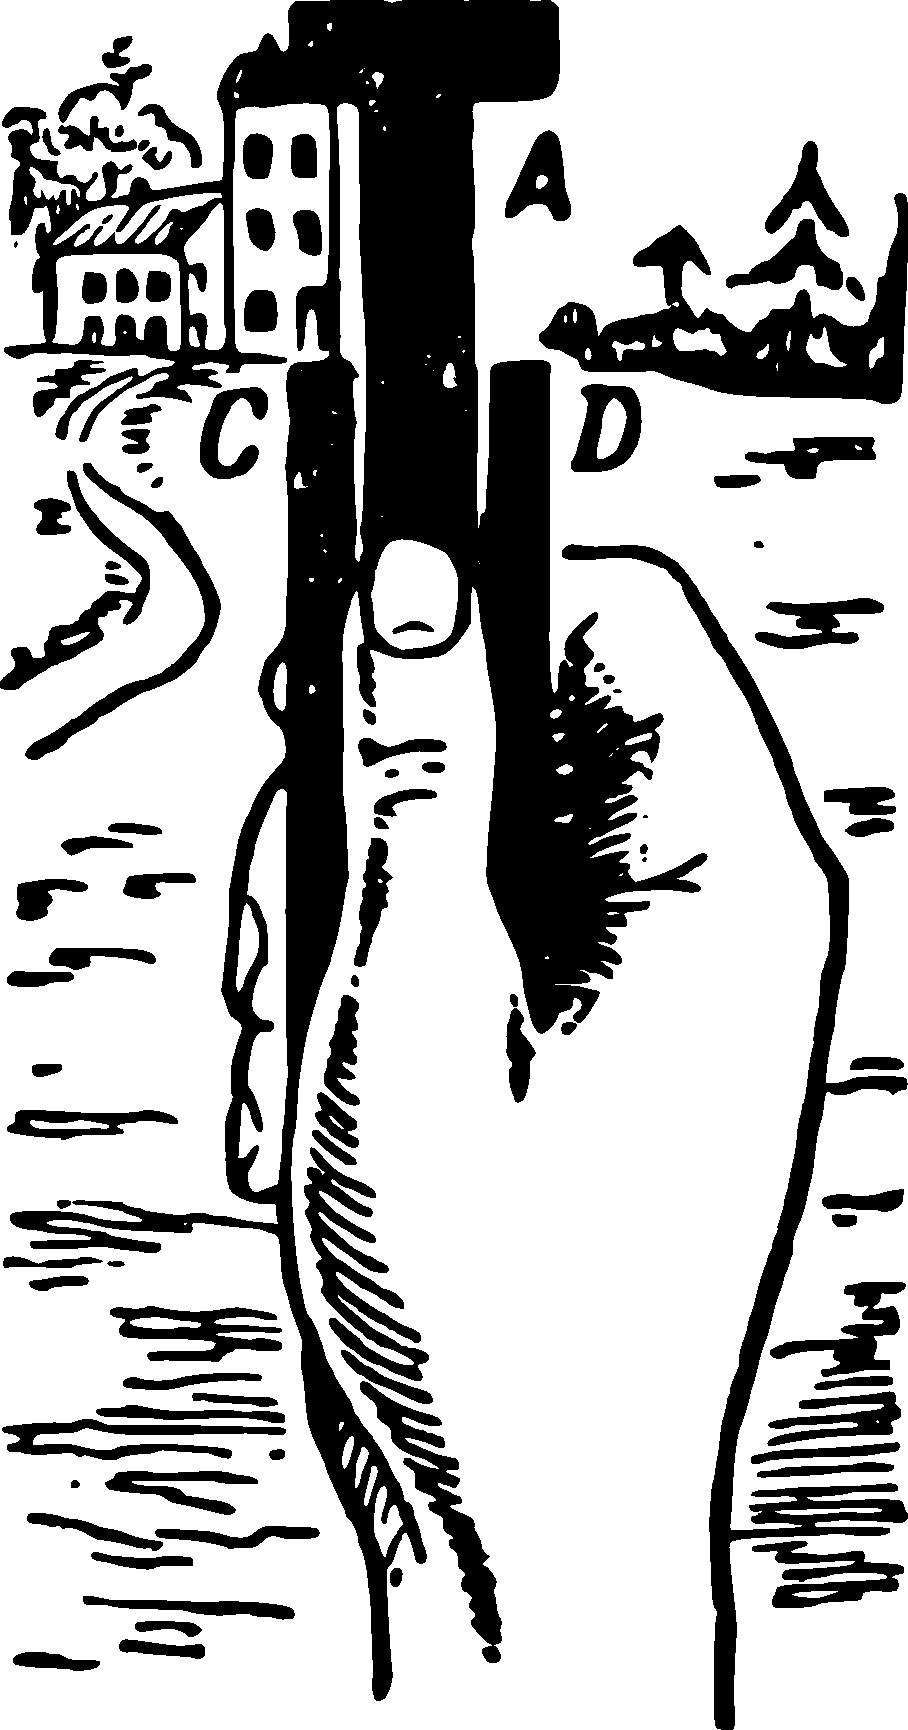
\includegraphics[width=0.8\textwidth]{figures/ch-02/fig-039.pdf}
\sidecaption{The retractable rangefinder in action.\label{fig-039}}
\end{marginfigure}

For those skilled in crafting, making a more convenient device of the same type, intended for estimating distances based on the size of a distant human figure, won't be much trouble.

\begin{marginfigure}%[-2cm]%[h!]
\centering
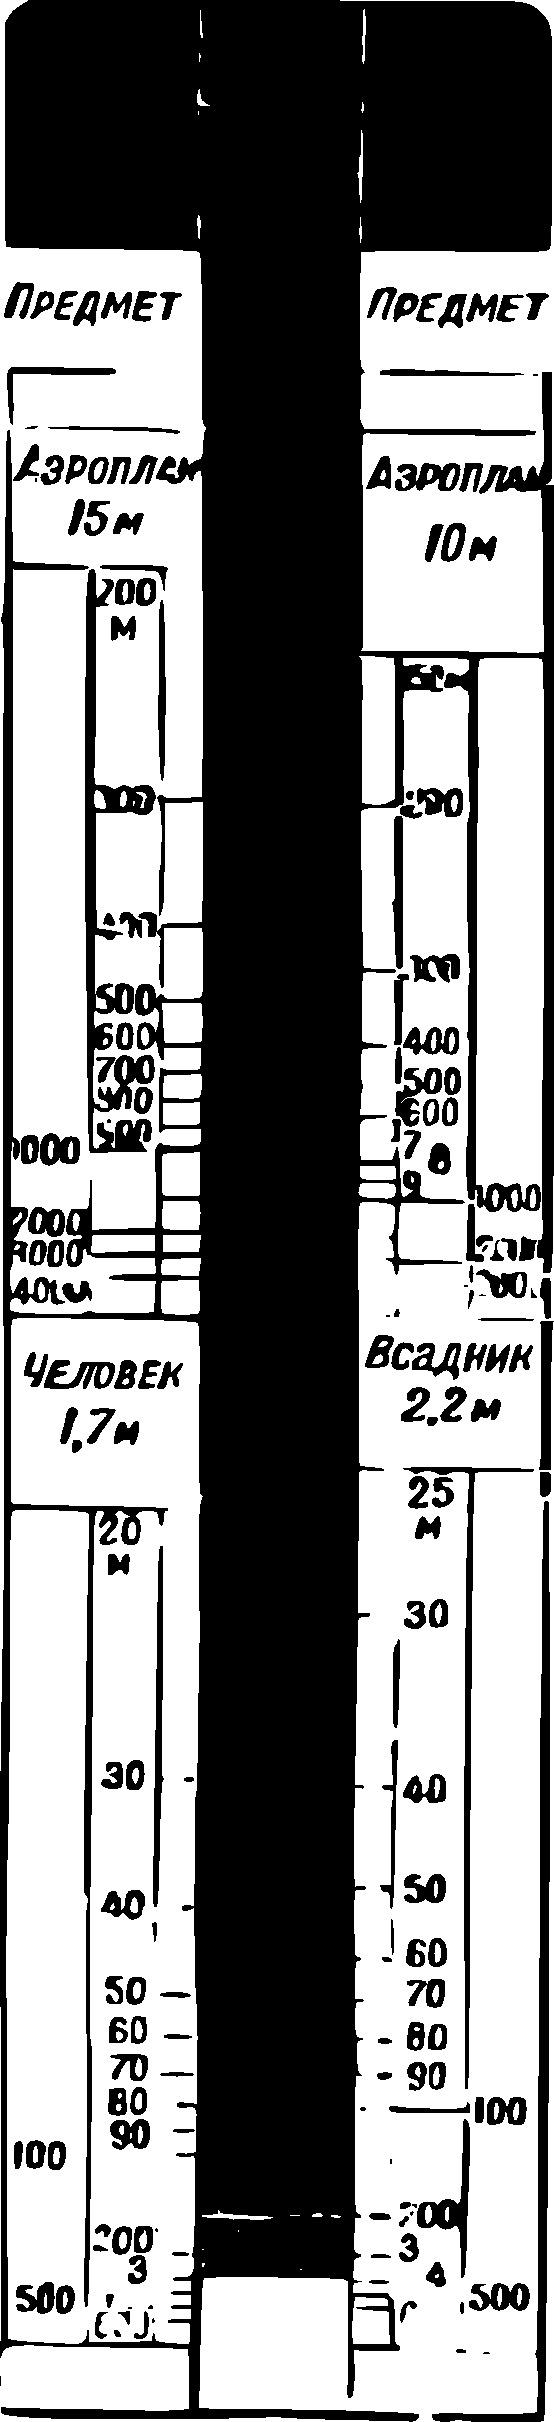
\includegraphics[width=0.6\textwidth]{figures/ch-02/fig-040.pdf}
\sidecaption{The design of the retractable rangefinder.\label{fig-040}}
\end{marginfigure}

The device is clear in \figr{fig-039} and \figr{fig-040}. The observed object is placed precisely in the gap $A$, formed when the extension part of the device is raised. The size of the gap can be conveniently determined by the divisions on the part $C$ and $D$ of the board. To avoid the need for any calculations, you can directly mark on strip $C$ the distances corresponding to the divisions if the observed object is a human figure (the device for measuring the distance of the outstretched arm). On the right strip $D$, you can mark distances, pre-calculated for cases where a rider is observed (\SI{2.2}{\meter}). For telegraph poles (height \SI{8}{\meter}), planes with a wingspan of \SI{15}{\meter}, and other larger objects, you can use the upper, free parts of strips $C$ and $D.$ Then the device will look like the one presented in \figr{fig-040}.





Of course, the accuracy of such distance estimation is low. It's just an estimate, not a measurement. In the example discussed earlier, where the distance to the human figure was estimated at \SI{85}{\meter}, an error of \SI{1}{\milli\meter} in measuring the matchstick portion would result in a deviation of \SI{7}{\meter} (1/12 out of 85). But if the person stood four times farther away, and we measured only \SI{3}{\milli\meter} on the matchstick, then an error of even 1/2 mm would cause a change in the result by \SI{57}{\meter}. Therefore, our example is reliable only for relatively short distances -- in the range of 100--200 m. When estimating larger distances, it's necessary to choose larger objects.


\section{The energy of the river}
\label{sec-2.6}

\begin{quote}
\emph{You know the edge where everything breathes abundance,\\
Where rivers flow purer than silver, \\
Where the steppe breeze sways the feather grass, \\
Where villages are nestled in cherry orchards.}\\[-10pt]
\flushright{\emph{A.K. Tolstoy}}
\end{quote}


A river, the length of which is no more than 100 km, is considered small. Do you know how many such small rivers there are in the USSR? A lot - 48 thousand!

If these rivers were stretched into a single line, it would result in a ribbon \SI{13800000}{\kilo\meter} long. With such a ribbon, you could encircle the Earth at the equator thirty times (the length of the equator is approximately \SI{40009}{\kilo\meter}).

The flow of these rivers is leisurely, but it conceals an inexhaustible supply of energy within it. Specialists believe that if the hidden potential of all the small rivers flowing through our homeland were combined, an impressive number would be obtained -- 34 million kilowatts! This gifted energy needs to be widely utilised for electrifying the economy of settlements located near rivers.

\begin{quote}
\emph{Let the river flow freely,\\
If the plan says so,\\
A dam with a stone ridge across all depths\\
Will block the way forever.}\\[-10pt]
\flushright{\emph{S. Shchipachev}}
\end{quote}

You know that this is achieved through hydroelectric power stations (HPS), and you can show a lot of initiative and provide real assistance in preparing for the construction of small HPS. Indeed, the builders of HPS will be interested in everything related to the river regime: its width and flow rate (``water flow''), the area of the cross-section of the riverbed (``active section''), and what water head the banks allow. And all this can be measured with available means and represents a relatively simple geometric problem.

We will now proceed to solving this problem.

But first, let's present here a practical advice from specialists, engineers V. Yarosh and I. Fedorov, regarding the selection of a suitable location on the river for the construction of a future dam.

They recommend building a small hydroelectric power station with a capacity of 15-20 kilowatts ``no further than 5 km from the village.''

``The dam of an HPS should be built no closer than 10-15 km and not farther than 20-40 km from the source of the river because moving away from the source entails the costly reinforcement of the dam, which is caused by a large influx of water. If the dam is located closer than 10-15 km from the source, due to the small water flow and insufficient head, the hydroelectric power station will not be able to provide the necessary power. The chosen stretch of the river should not be abundant in great depths, which also increases the cost of construction, requiring a heavy foundation.''

\section{The Flow Rate}
\label{sec-2.7}
\begin{quote}
\emph{Between village and mountain grove,\\
Winds a river like a bright ribbon.}\\[-10pt]
\flushright{\emph{A. Fet}}
\end{quote}

How much water flows in such a river in a day? It's easy to calculate if you first measure the speed of the water flow in the river. The measurement is performed by two people. One person holds a watch, the other holds some noticeable float, for example, a half-empty bottle with a flag. They choose a straight section of the river and place two stakes $A$ and $B$ along the bank at a distance, for example, \SI{10}{\meter} from each other (see \figr{fig-041}).

\begin{figure}[h!]
\centering
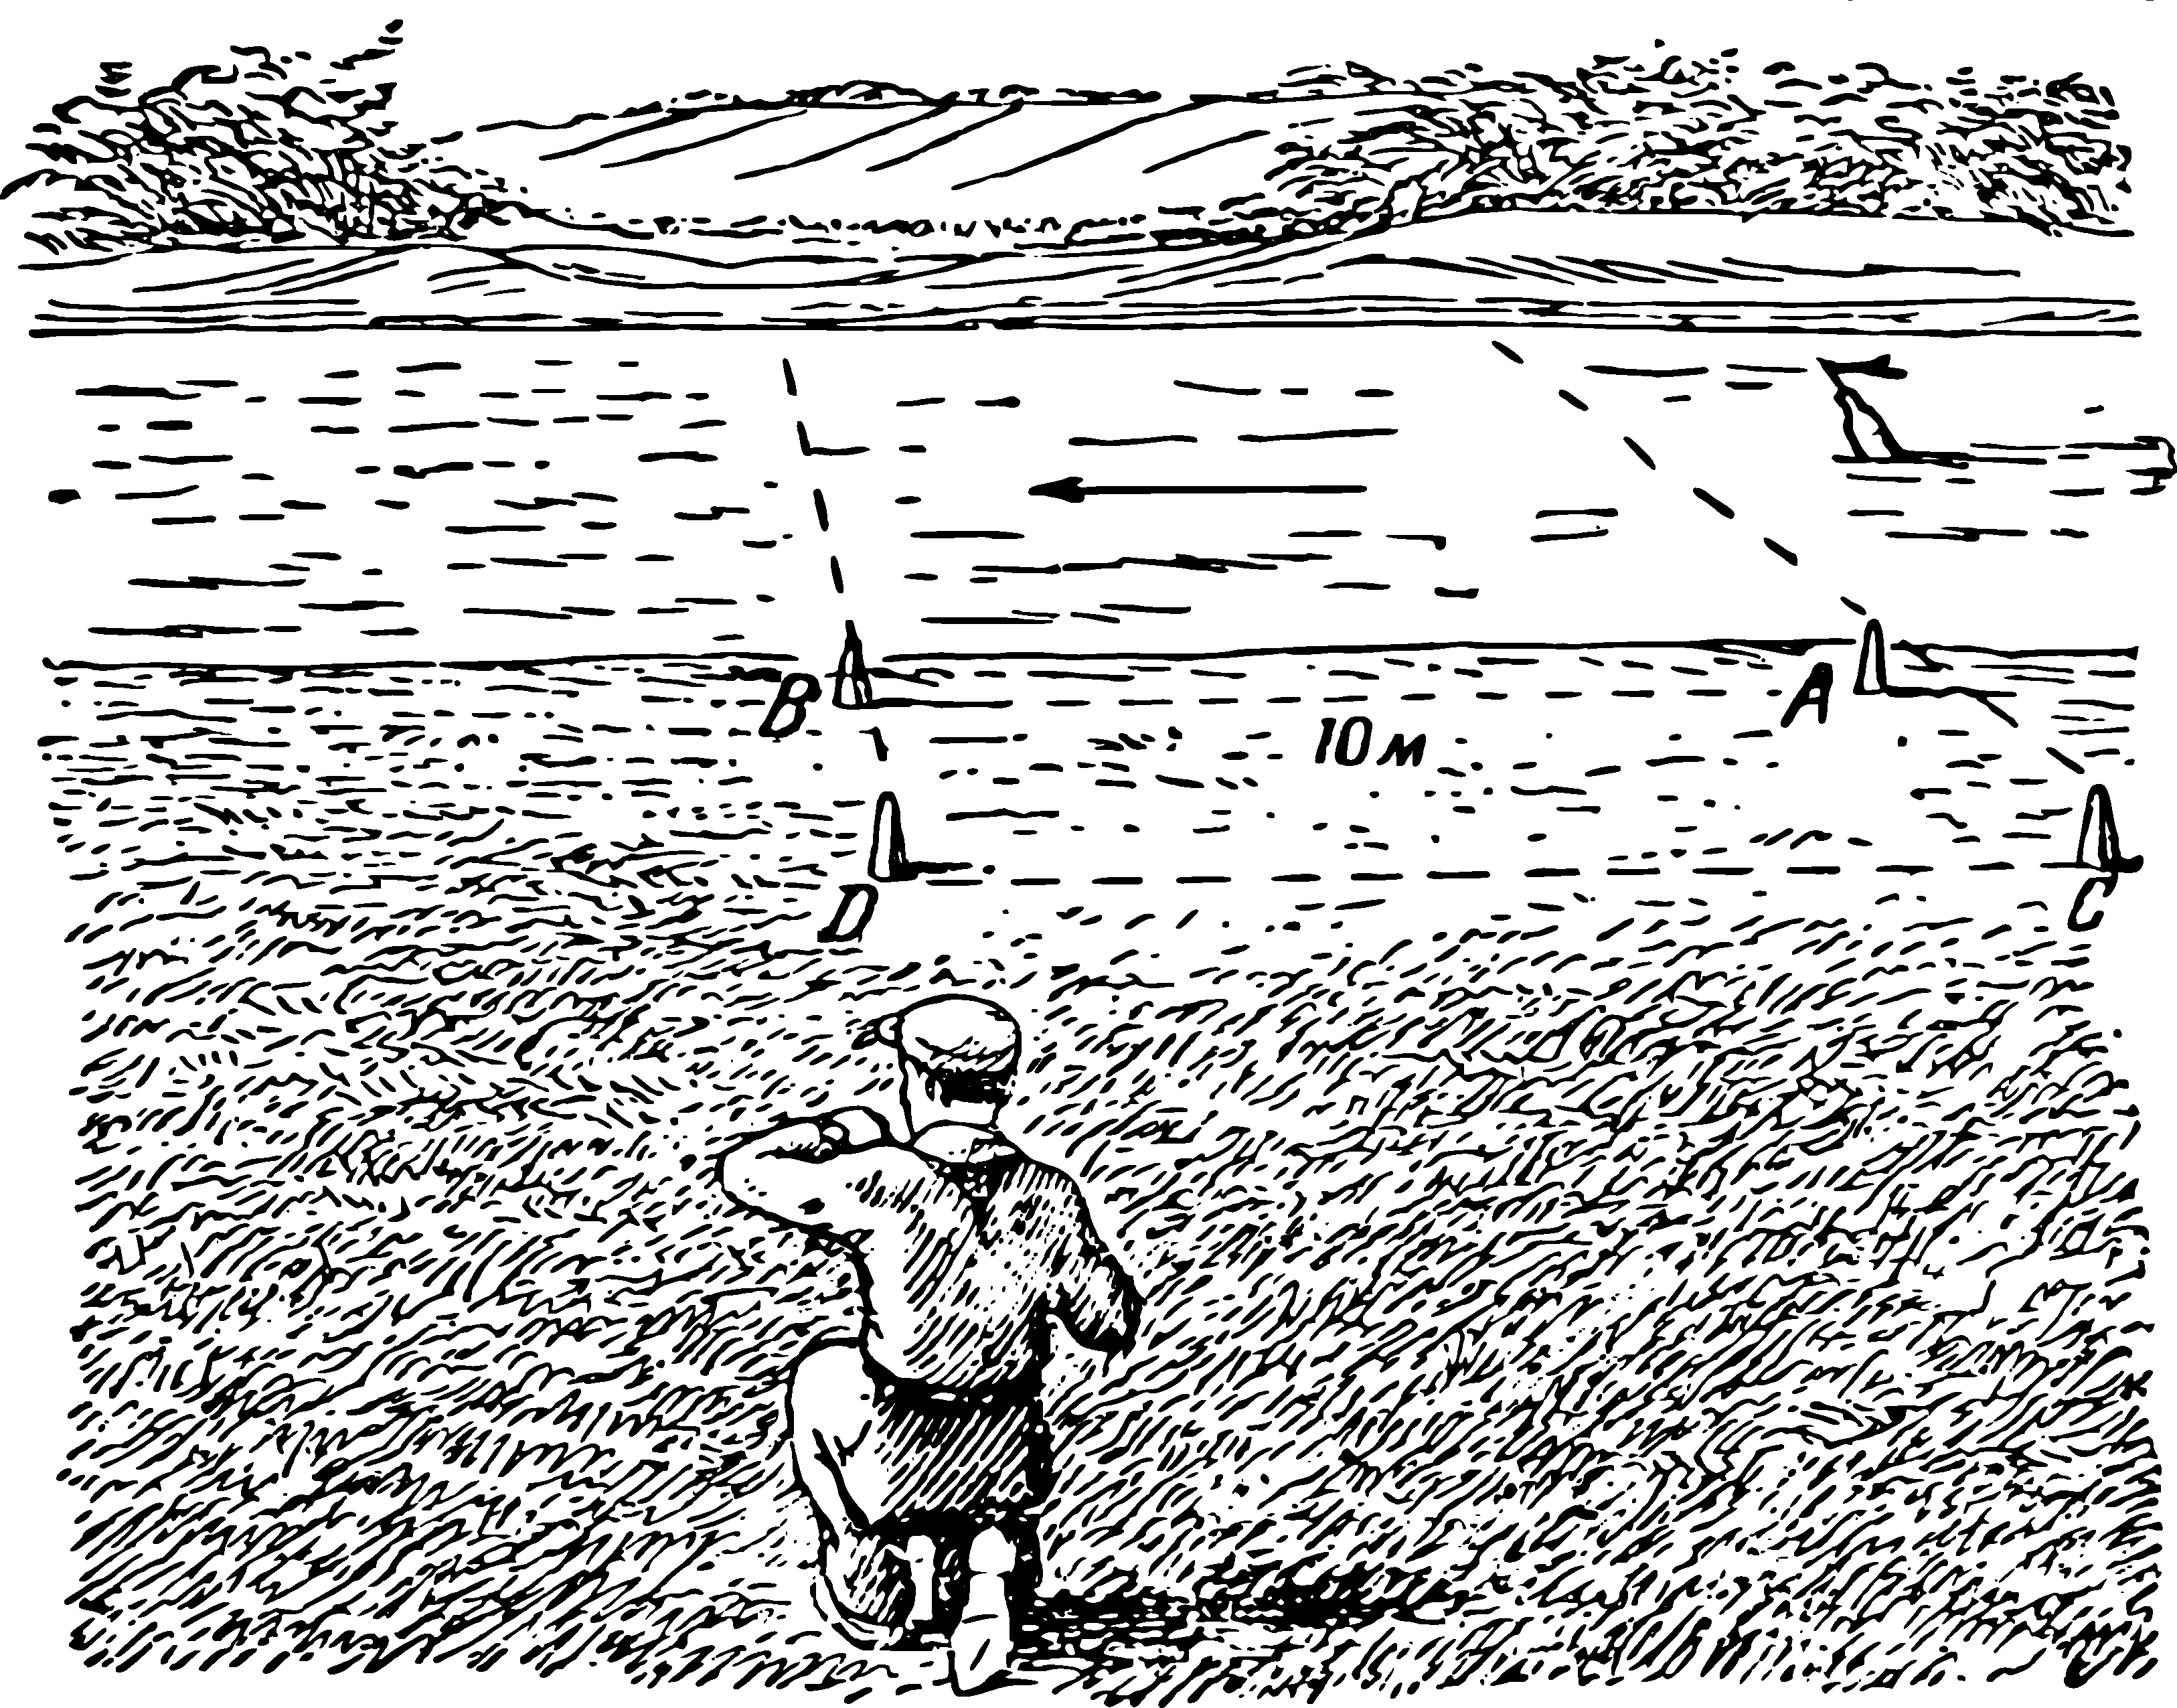
\includegraphics[width=0.9\textwidth]{figures/ch-02/fig-041.pdf}
\sidecaption{Measurement of the river flow velocity.\label{fig-041}}
\end{figure}

Two more stakes $C$ and $D$ are placed on lines perpendicular to $AB$. One of the participants in the measurement with the watch stands behind stake $D$. The other, with the float, goes a bit upstream of stake $A$, throws the float into the water, and then stands behind stake $C$. Both observers look along the directions $CA$ and $DB$ towards the water surface. At the moment when the float crosses the extension of the line $CA$, the first observer waves his hand. Upon this signal, the second observer starts the timer for the first time and then again when the float crosses the direction of $DB$.

Let's assume that the time difference is 20 seconds.

Then the speed of the water flow in the river is:
\begin{equation*}%
\frac{10}{20} = \SI{0.5}{\meter\per\second}.
\end{equation*}
Usually, the measurement is repeated about ten times\sidenote{Instead of throwing one float ten times, you can immediately throw 10 floats at some distance from each other.}, throwing the float into different points on the river surface. Then the obtained numbers are summed up and divided by the number of measurements. This gives the average speed of the surface layer of the river.

Deeper layers flow slower, and the average speed of the entire flow is approximately 4/5 times the surface speed. In our case, therefore, it's \SI{0.4}{\meter\per\second}.

You can determine the surface speed by another -- albeit less reliable -- method.

Sit in a boat and paddle \SI{1}{\kilo\meter} (measured along the shore) against the current, and then back -- with the current, trying to paddle with the same force all the time.

Let's say you paddled these \SI{1000}{\meter} against the current in 18 minutes, and with the current in 6 minutes. Denoting the desired speed of the river current as $x$, and the speed of your movement in still water as $y$, you form the equations:
\begin{equation*}%
\frac{1000}{y - x} = 18, \qand \frac{1000}{y + x} = 6.
\end{equation*}
Rearranging we get:
\begin{equation*}%
y + x = \frac{1000}{6}, \qand y - x = \frac{1000}{18}.
\end{equation*}
Solving for $x$, we get $2x = 110$, and $x = 55$. The speed of the water flow on the surface is 55 m per minute, and therefore, the average speed is about 5/6 \si{\meter\per\second}.


\section{How Much Water Flows In The River?}


To measure the amount of water flowing in a river, you can always determine the speed at which the water flows. The more challenging part of the preparatory work needed to calculate the quantity of flowing water is to determine the cross-sectional area of the water. To find the magnitude of this area, known as the ``live cross-section'' of the river, you need to make a drawing of this section. Such work is done as follows.

\textbf{First Method:} At the point where you measured the width of the river, you drive a stake into the ground on both banks, right at the water's edge. Then, with a companion, you get into a boat and row from one stake to the other, trying to keep a straight line connecting the stakes. An inexperienced rower will not be able to handle such a task, especially in a river with a fast current. Your companion must be a skilled rower; besides, a third participant in the work should stand on the bank, ensuring that the boat stays on the correct course and giving the rower signals indicating which way to turn when necessary. During the first crossing of the river, you only need to count how many strokes of the oars it took and from there figure out how many strokes move the boat 5 or 10 meters. Then, for the second crossing, armed with a sufficiently long rake with markings on it, you plunge the rake vertically to the bottom every 5-10 meters (measured by the number of oar strokes) and record the depth of the river at that point.

This method can only measure the live cross-section of a small river; for a wide, multi-water river, more complex methods are needed, which are performed by specialists. An amateur must choose a task that suits their modest measuring means.

\textbf{Second Method:} On a narrow and shallow river, you don't need a boat.

Between the stakes, you stretch a cord perpendicular to the current with marks or knots made on it every 1 or 2 meters, and by lowering a ruler to the bottom at each knot, you measure the depth of the riverbed. When all measurements are done, you first draw a millimeter paper or a grid paper sketch of the cross-section profile of the river. You will get a figure similar to the one shown in \figr{fig-042}. It is quite easy to determine the area of this figure since it can be divided into a series of trapezoids (where both bases and the height are known) and two side triangles, also with known base and height. If the scale of the drawing is 1:100, then the result will be obtained directly in square meters.

\begin{figure}[h!]
\centering
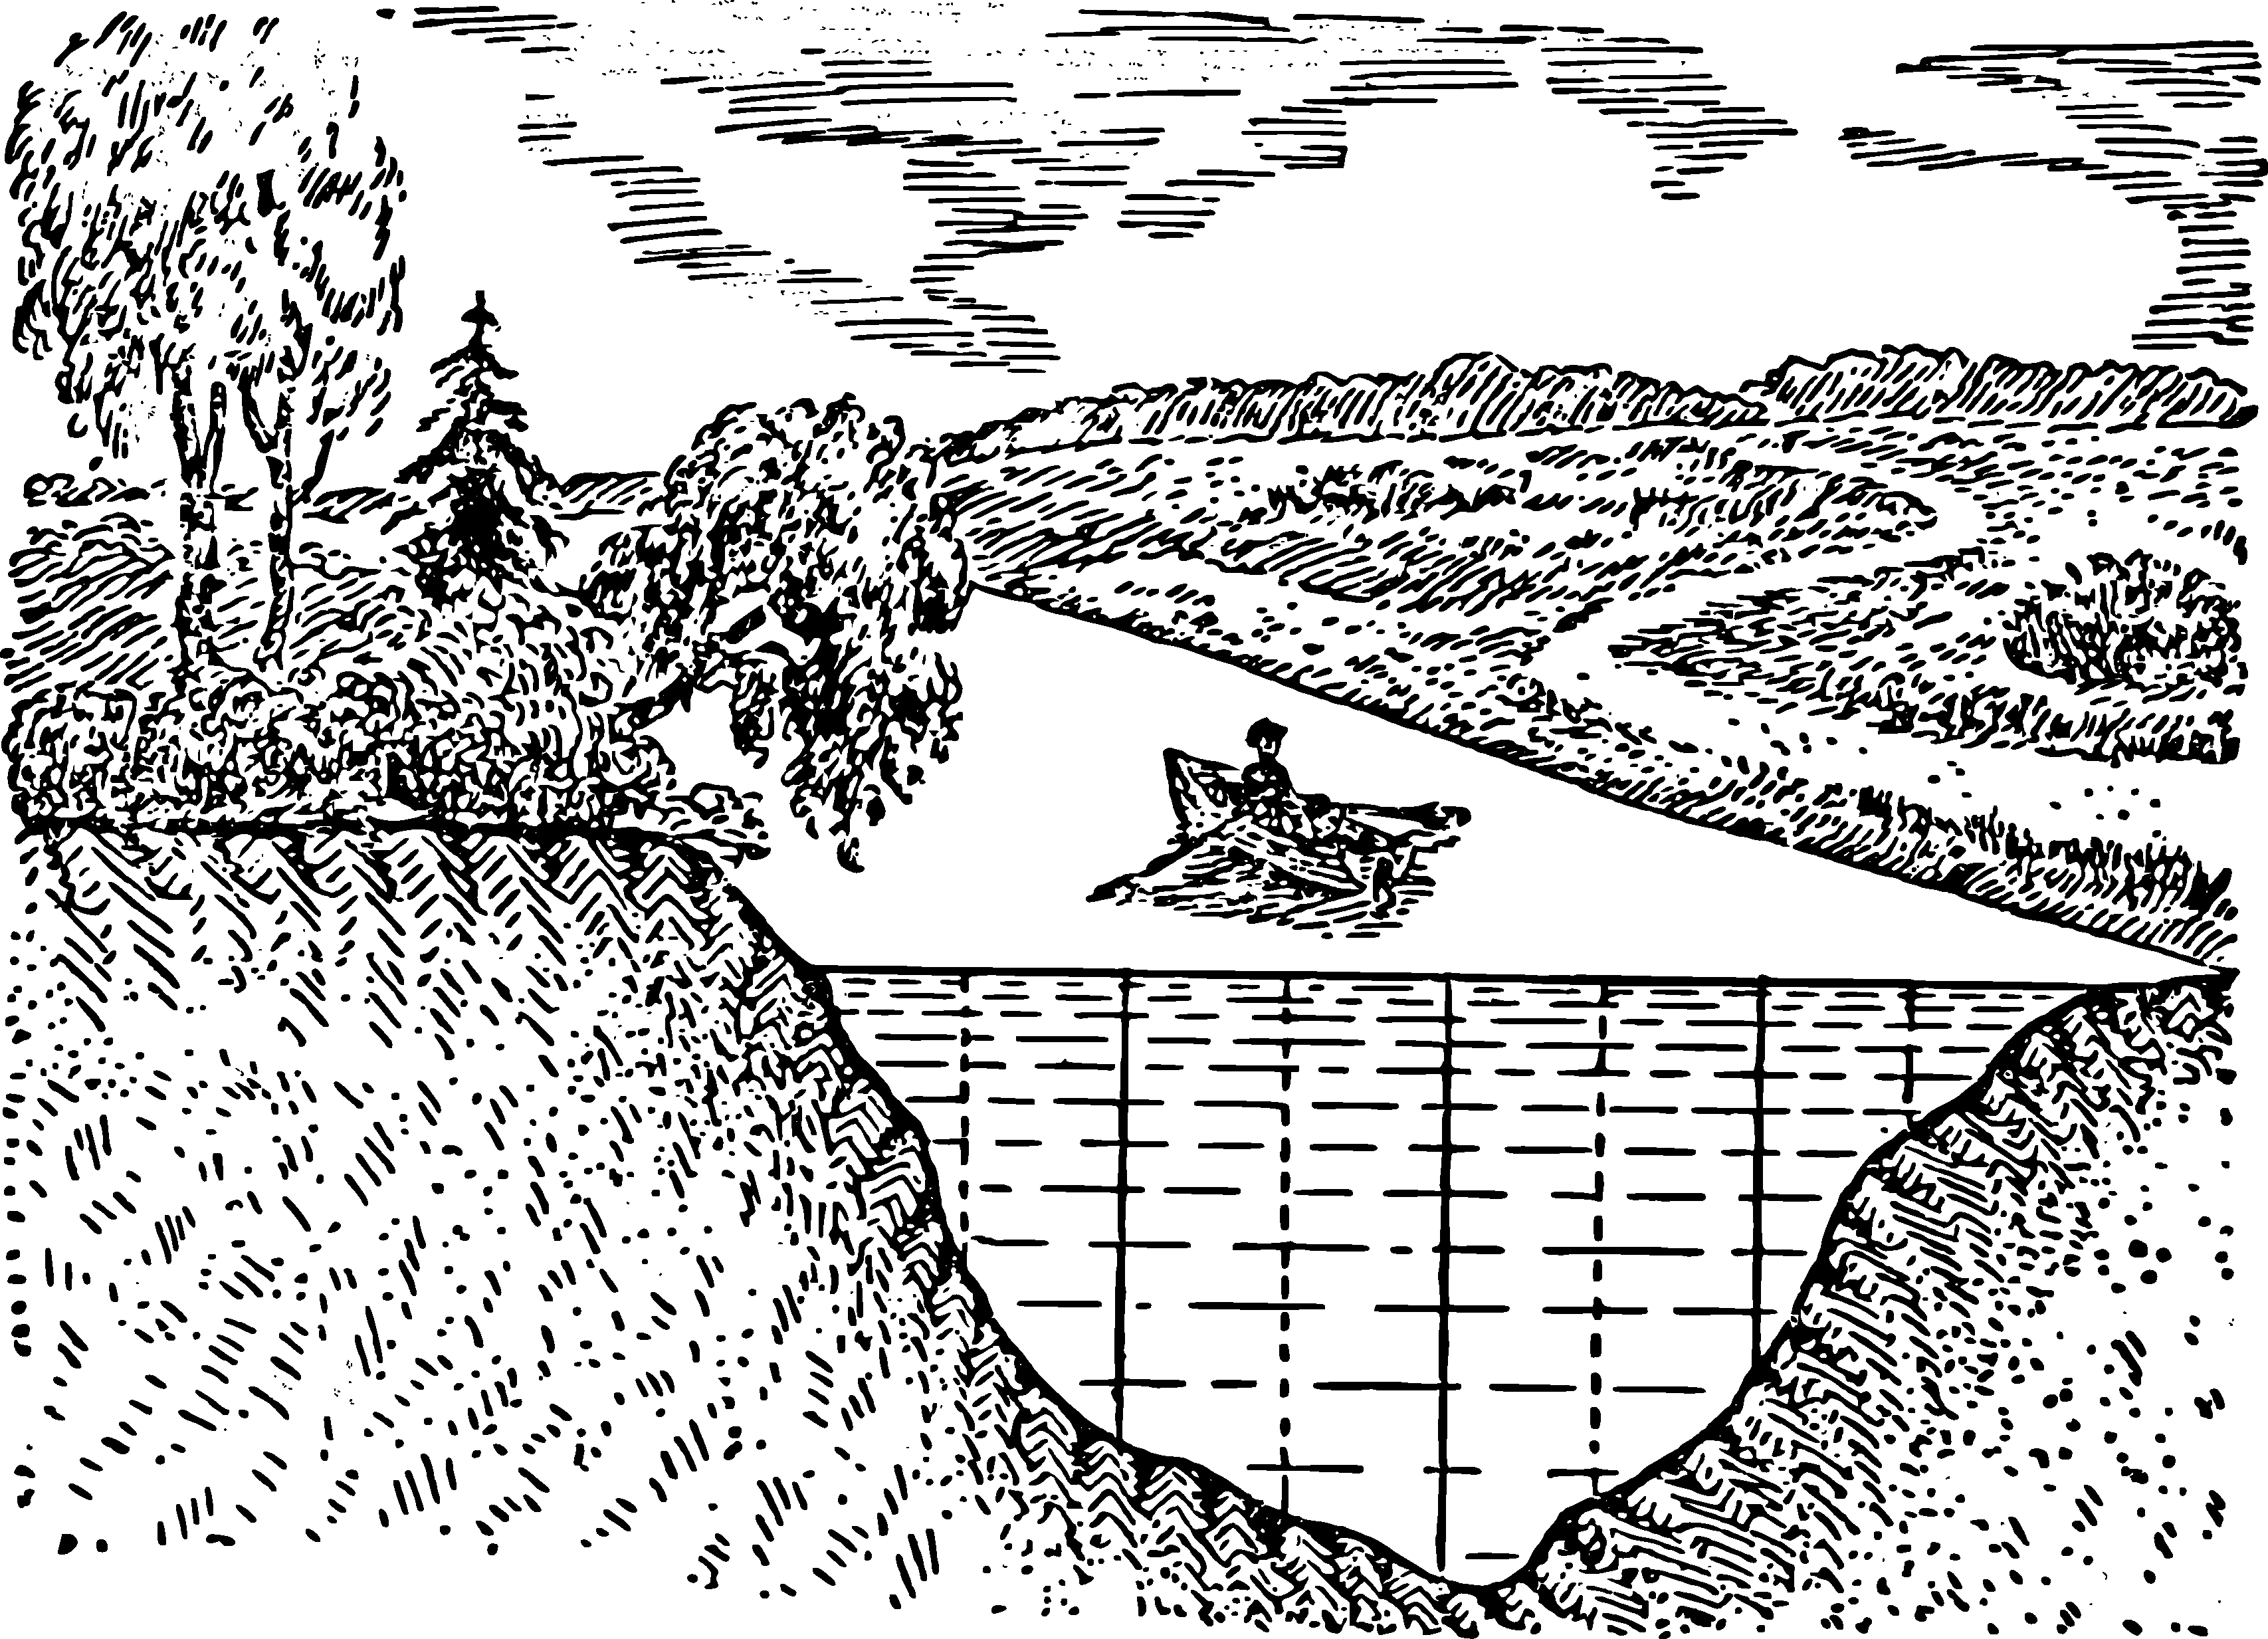
\includegraphics[width=0.9\textwidth]{figures/ch-02/fig-042.pdf}
\sidecaption{``Live Cross-Section'' of a River.\label{fig-042}}
\end{figure}

Now you have all the data needed to calculate the amount of flowing water. Obviously, through the live cross-section of the river, a volume of water equal to the volume of a prism is passing every second, where the cross-section serves as the base and the average second-by-second flow rate serves as the height. For example, if the average flow rate of water in the river is 0.4 meters per second, and the area of the live cross-section is, let's say, 3.5 square meters, then every second, through this section, there will be a transfer of

3.5 * 0.4 = 1.4 cubic meters of water,

or the same amount in tons. This amounts to 1.4 x 3600 = 5040 cubic meters per hour, and 5040 x 24 = 120960 cubic meters per day, which is over a hundred thousand cubic meters. And yet, a river with a wetted cross-section of 3.5 square meters is a small river; it could be, for example, 3.5 meters wide and 1 meter deep at a fordable point. But even it contains energy capable of transforming into mighty electricity. So how much water flows per day in a river like the Neva, through which 3300 cubic meters of water pass every second through its wetted cross-section! This is the 'average flow rate' of water in the Neva at Leningrad. The 'average flow rate' of water in the Dnieper at Kiev is 700 cubic meters.

Young explorers and future dam builders also need to determine the maximum head the banks can allow, i.e., the difference in water levels that the dam can create (Fig. 43). To do this, stakes are driven into the banks 5-10 meters away from the water, as usual, along a line perpendicular to the river's current. Then, moving along this line, small stakes are placed at points of characteristic bends in the banks (Fig. 44). Using rulers with markings, the elevation of one stake above the other and the distances between them are measured. Based on the measurement results, a profile of the banks is drawn similar to the profile of the riverbed. The bank profile can indicate the magnitude of the allowable head.

Suppose the water level can be raised by the dam by 2.5 meters. In this case, you can estimate the potential power of your future hydroelectric power plant.

For this, energy experts recommend multiplying 1.4 (the second-by-second flow rate of the river) by 2.5 (the water level height) and by 6 (the coefficient, which varies depending on energy losses in machines). The result will be in kilowatts. Thus,

1.4 x 2.5 x 6 = 21 kilowatts.

Since the river levels, and consequently the flow rates, vary throughout the year, it is necessary to calculate the value of the flow rate that is characteristic of the river for most of the year."

%\begin{center}
%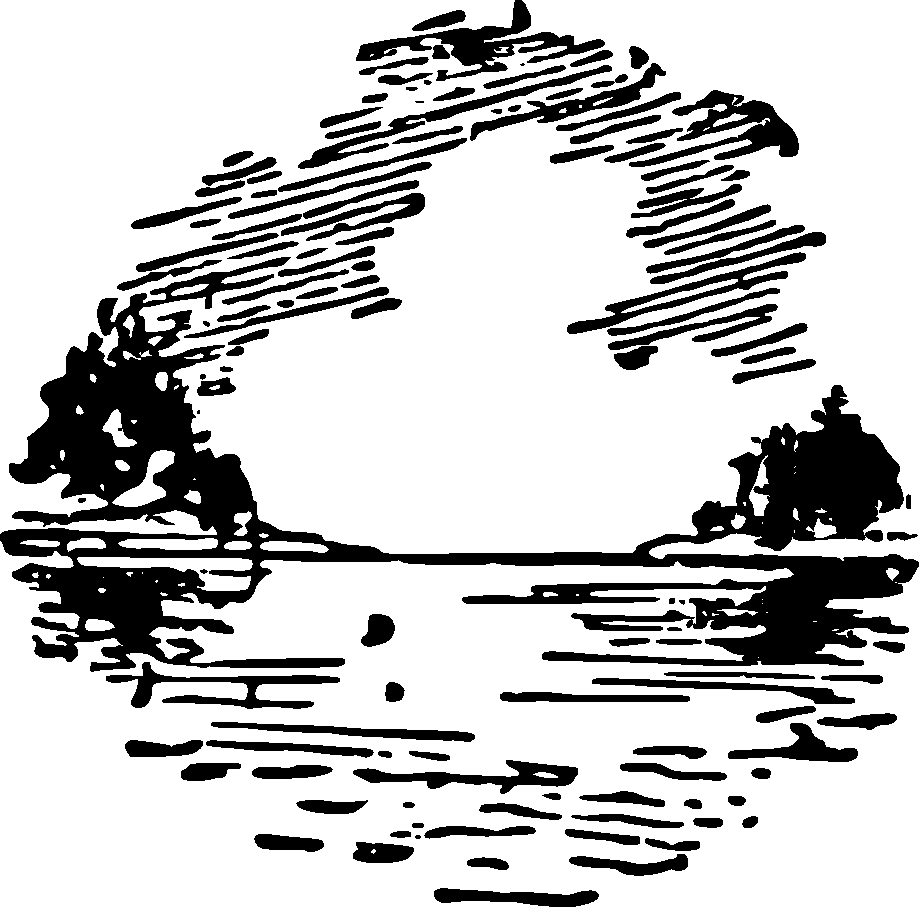
\includegraphics[width=0.3\textwidth]{figures/ch-02/fig-ch-02-tail.pdf}
%\end{center}


















